\setcounter{excounter}{1}
\setcounter{examplecounter}{1}
\chapter{Conditionals, Recursion, and Loops}
\label{chapter-crl} % Always give a unique label
% use \chaptermark{}
% to alter or adjust the chapter heading in the running head

\abstract*{Each chapter should be preceded by an abstract (no more than 200 words) that summarizes the content. The abstract will appear \textit{online} at \url{www.SpringerLink.com} and be available with unrestricted access. This allows unregistered users to read the abstract as a teaser for the complete chapter.
Please use the 'starred' version of the new \texttt{abstract} command for typesetting the text of the online abstracts (cf. source file of this chapter template \texttt{abstract}) and include them with the source files of your manuscript. Use the plain \texttt{abstract} command if the abstract is also to appear in the printed version of the book.}

\abstract{Each chapter should be preceded by an abstract (no more than 200 words) that summarizes the content. The abstract will appear \textit{online} at \url{www.SpringerLink.com} and be available with unrestricted access. This allows unregistered users to read the abstract as a teaser for the complete chapter. \newline\indent
Please use the 'starred' version of the new \texttt{abstract} command for typesetting the text of the online abstracts (cf. source file of this chapter template \texttt{abstract}) and include them with the source files of your manuscript. Use the plain \texttt{abstract} command if the abstract is also to appear in the printed version of the book.}

\section{Conditionals}

Decisions are otherwise called \emph{conditionals}. We have seen conditionals before, but in this section we will reintroduce them as a concept and discuss the intricacies of Java's conditionals, including the different logical operators and behaviors thereof.

In Java, we use \ttt{if} to designate a branch in code. We supply to it a conditional expression, or a \emph{predicate}\index{predicate}, which resolves to either true or false. In essence, predicates resolve to boolean values. For example, if we want to return $5$ if two integers $a$ and $b$ are the same value, we write the following:
\begin{lstlisting}[language=MyJava]
static int foo() {
  int a = ...;
  int b = ...;
  if (a == b) { return 5; }
  return 0;
}
\end{lstlisting}
The \ttt{==} operator compares primitive values for equality, as we stated in our Java primer. If we want to use the result of a (boolean) method as the condition, we might want to inline the invocation. 
%\enlargethispage{-2\baselineskip}
\begin{lstlisting}[language=MyJava]
static boolean bar() {
  ...
}

static int foo() {
  if (bar()) { return 5; }
  return 0;
}
\end{lstlisting}
We negate conditional expressions using the exclamation point operator, i.e., \ttt{!}. That is, if $e$ is an expression that returns a boolean value, $\ttt{!}e$ flips the output value from true to false or vice versa. We can chain conditional expressions together using the logical AND/OR operators, namely \ttt{\&\&} and \ttt{||} respectively. All boolean subexpressions that comprise a larger expression, conjoined by \ttt{\&\&}, must be true for the overall expression to be true. On the other hand, when boolean expressions are conjoined by \ttt{||}, only one must be true. 

Both logical AND and logical OR are called \emph{short-circuiting operators}. Regarding the former, if we have the expression $e = e_1 \;\ttt{\&\&}\;e_2$, and $e_1$ resolves to false, then $e_2$ is not evaluated, because both operands must be true for the result of the AND to be true. Logical OR works similarly; if we have the expression $e = e_1\;\ttt{||}\;e_2$, and $e_1$ resolves to true, then $e_2$ is not evaluated, because only one operand has to be true for the result of the OR to be true.

\begin{lstlisting}[language=MyJava]
static int foo() {
  int a = 5;
  int b = 10;
  int c = 5;
  // We never check if c == 5.
  if (a == b && c == 5) { return 100; }
  // We never check if b != 10.
  if (a == c || b != 10) { return 200; }
  return 0;
}
\end{lstlisting}

In addition to \ttt{if}, Java also has \ttt{else} and \ttt{else if} for extending the possible outcomes of a condition. When the predicate of a preceding \ttt{if} is false and an \ttt{else} block is attached, its code is evaluated. Moreover, when the predicate of a preceding \ttt{if} is false and an \ttt{else if} block is attached, the condition to the \ttt{else if} is evaluated. The former pairing represents a binary outcome, whereas the latter corresponds to more than two possible outcomes. Multiple \ttt{if} statements ``stacked above one another'' results in their sequential evaluation since Java assumes they are disjoint code segments. The \ttt{else if} block, on the contrary, executes only when its preceding \ttt{if} condition resolves to false. In the following code listing, we show an example of two sets of conditional statements; the former uses only \ttt{if} and the latter takes advantage of \ttt{if}, \ttt{else if}, and \ttt{else}. Accordingly, the left-hand listing returns $20$ and the right-hand listing returns $10$.

\begin{clrr}[]{}
\begin{lstlisting}[language=MyJavaNF]
static int foo() {
  int x = 10;
  int y = 0;
  if (x == 10) { y=5; } 
  if (y == 5) { y+=10; }
  if (x != 10 && y != 5) { y+=5; }
  return y;
}
\end{lstlisting}
\tcblower
\begin{lstlisting}[language=MyJavaNF]
static int foo() {
  int x = 10;
  int y = 0;
  if (x == 10) { y=10; } 
  else if (y == 5) { y+=10; } 
  else { y+=5; }
  return y;
}
\end{lstlisting}
\end{clrr}

\myexample{Suppose we want to translate a \ttt{String} grade into its grade-point average equivalent, treating pluses and minuses as grade increment or decrements. Our grading schema has no grade higher than a $4.0$, and all failing grades result in a zero. After writing the tests, we can use a series of \ttt{if} and \ttt{else if} statements as a case analysis on the letter grade. Afterwards, once we have the base GPA according to the letter, we apply the plus or minus given the aforementioned criteria. When determining the initial GPA value, were we to use a series of \ttt{if} statements as opposed to \ttt{if}/\ttt{else if}/\ttt{else}, every predicate would need to be evaluated regardless of whether it is meaningful. By ``meaningful,'' we mean to suggest that, for instance, once we know the GPA is a 4.0, it makes no sense to determine if the grade is a \ttt{`B'}, since we know from the previous branch that it is an \ttt{`A'}. The \ttt{else if} statements are skipped over if a preceding condition resolves to true.}


\begin{lstlisting}[language=MyJava]
import static Assertions.assertAll;
import static Assertions.assertEquals;

class GpaCalculatorTesting {

  @Test
  void testGpa() {
    assertAll(
      () -> assertEquals(4.0, gpa("A+")),
      () -> assertEquals(3.7, gpa("A-")),
      () -> assertEquals(0.0, gpa("F-")));
  }
}
\end{lstlisting}

\begin{lstlisting}[language=MyJava]
class GpaCalculator {

  /**
   * Computes the numeric GPA for a given letter grade.
   * @param letter - grade between A and F, with optional +/-.
   * @return numeric grade from 4.0 to 0.0.
   */
  static double gpa(String grade) {
    boolean plus = grade.contains("+");
    boolean minus = grade.contains("-");
    char letter = grade.charAt(0);
    double gpa = 0;
    
    // Compute the grade letter.
    if (letter == 'A') {  gpa = 4.0; } 
    else if (letter == 'B') { gpa = 3.0; } 
    else if (letter == 'C') { gpa = 2.0; } 
    else if (letter == 'D') { gpa = 1.0; } 
    else { gpa = 0.0; }
    
    // Compute +/- if applicable.
    if (letter != 'A' && letter != 'F') { gpa = plus ? gpa + 0.3 : gpa; }
    if (letter != 'F') { gpa = minus ? gpa - 0.3 : gpa; }
    return gpa;
  }
}
\end{lstlisting}

The latter two \ttt{if} statements, as we said, apply increments or decrements based on whether the grade is a \ttt{+} or a \ttt{-}. We use the not-equal-to operator, \ttt{!=}, to circumvent having to apply a negation on the outside, i.e., \ttt{!(letter == `A')}. The bodies of these cases, however, appear to be foreign, and indeed, we introduce the \emph{ternary operator}. Because \ttt{if} is a statement, there is no way to inline a conditional into an expression. The ternary operator is a fix to this problem. We read ${r = p\;?\;c\;:\;a}$ as follows: ``if $p$ is true, assign $c$ to $r$, otherwise assign $a$ to $r$.'' Inlining conditional expressions in this fashion reduces code clutter but should be used sparingly. We could write all \ttt{if} statements as ternary operations, but doing so would obfuscate our logic.

Aside from the `\ttt{if}'/`\ttt{else if}'/`\ttt{else}' trio, plus the ternary operator, Java has the \ttt{switch}/\ttt{case} statements, which serve to help simplify case analysis problems. A \ttt{switch} statement receives an expression $e$ that resolves to some value $v$. Inside the \ttt{switch} exists \ttt{case} statements, corresponding to possible outcomes of $e$'s evaluation. For instance, if we wanted to write a method that determines the number of days there are in a given (non-leap year) month, we might be inclined to use several \ttt{if} statements, which is prone to errors. Let us see the answer to this problem using \ttt{switch} and \ttt{case} statements.

\begin{lstlisting}[language=MyJava]
import static Assertions.assertAll;
import static Assertions.assertEquals;

class MonthToDaysTester {

  @Test
  void testMonthToDays() {
    assertAll(
      () -> assertEquals(31, monthToDays("January")),
      () -> assertEquals(28, monthToDays("February")),
      () -> assertEquals(31, monthToDays("May")),
      () -> assertEquals(31, monthToDays("July")),
      () -> assertEquals(31, monthToDays("August")),
      () -> assertEquals(30, monthToDays("September")),
      () -> assertEquals(31, monthToDays("December")));
  }
}
\end{lstlisting}

\begin{lstlisting}[language=MyJava]
class MonthToDays {

  /**
   * Determines how many days a given month has, 
   * not accounting for leap years.
   * @param m - capitalized month, e.g., "July".
   * @return the number of days in the month
   */
  static int monthToDays(String m) {
    int days = 0;
    switch (m) {
      case "February":
        days = 28;
        break;
      case "April":
      case "June":
      case "September":
      case "November":
        days = 30;
        break;
      default:
        days = 31;
    }
    return days;
  }
}
\end{lstlisting}

We evaluate $m$ inside the \ttt{switch} statement, and it resolves to one of twelve possible strings, assuming the input is a valid and capitalized month. If, for instance, the string is \ttt{"February"}, we assign $\mathit{days}$ to $28$ and perform a \ttt{break}. Cases that comprise a \ttt{switch} block can ``fall through'' to the next case, meaning that if we did not insert a \ttt{break}, the program would fall all the way to the \ttt{default} case and assign $31$ to $\mathit{days}$. Default cases correspond to ``anything other data,'' similar to \ttt{else} blocks. In our case, we place all months that have thirty-one days in the default case to reduce the number of lines in our code. In the case of a month having thirty days, there are four possibilities, and we stack these atop one another to state that these months should have $30$ assigned to $\mathit{days}$. If we wanted to omit the \ttt{break} statements, we might instead inline \ttt{return} statements directly, since we do not do anything aside from return $\mathit{days}$ at the end of the method. Of course, this solution only works when the resulting target of a \ttt{switch} block \emph{is} the desired value.
\section{Recursion}

In this section we reintroduce recursion as a means of problem decomposition and repetition. We present two forms: standard recursion and tail recursion, as well as the issues that come with both in Java. The discussion starts with a review of basic arithmetic and how it is translatable into recursion.

\subsection{Standard Recursion}
You may or may not have seen recursion before, but in theory the concept is quite simple: a method $f$ is \emph{recursive} if, somewhere in the definition of \emph{f}, it invokes itself. For example, in the following code segment, we define $f$ to be a method of arbitrary arguments that calls itself from its body. 
\begin{verbnobox}[\small]
static int f(...) {
  ...
  f(...);
  ...
}
\end{verbnobox}
Some may question the need for recursive methods, as it appears to be circular; why would we ever want a method to call itself? There are two reasons, where the former is what we consider to be less significant than the latter:

\begin{enumerate}
    \item It allows the programmer to repeat a given segment of code.
    \item We can compose the solution to a big problem by combining the solutions to smaller problems.
\end{enumerate}
So, we may certainly use recursion to repeat a task and, by transitivity, we will do that, but we primarily write recursive methods to solve some large problem by breaking it down into smaller problems that we know how to solve.

\myexample{Let us consider the question of addition. Consider a context where we have access to only three methods: \ttt{addOne}, \ttt{subOne}, and \ttt{isZero}, all of which are trivially defined. We also have access to conditional statements and method calls. Finally, we have an identity that $m + 0 = m$ for any natural number $m$. Here's the problem that we want to solve: we want to add two natural numbers $m$ and $n$, but how do we do that? Think about how humans calculate the sum of two natural numbers (perhaps some do it differently from others, but the general process is the same). Since we do not have a \ttt{+} operator in this context, we have to try a different approach. Recall the identity that we have at our disposal: $m + 0 = m$. Is there a way we can make use of the identity? Imagine that we want to solve $3 + 4$ in this context. Can we rewrite this expression that takes advantage of those methods that we have at our disposal? Indeed, we can rewrite this as a series of calls to \ttt{subOne} and \ttt{addOne}, but we will first show this in math notation.}
\begin{align*}
    &= 3 + 4\\
    &= (3 + 3) + 1\\
    &= ((3 + 2) + 1) + 1)\\
    &= (((3 + 1) + 1) + 1) + 1\\
    &= ((((3 + 0) + 1) + 1) + 1) + 1
\end{align*}
To solve $3 + 4$, we need to solve $3 + 3$, which means we need to solve $3 + 2$, which means we need to solve $3 + 1$, which means we need to solve $3 + 0$. Substituting $3$ for $m$ gives us the identity, meaning this expression resolves to $m$, namely $3$. Recursively breaking down a problem into smaller problems is called \emph{invoking the recursion}. Namely, we invoke the function of interest, \ttt{+}, inside its own definition. As part of this, we decrement $n$ by one in attempt to head towards the identity, or the problem that we know how to solve. Such a problem is called the \emph{base case} to our recursive method. How do we know what the base case is for this particular problem? We use our predicate for detecting if a value is zero, of course.

We still have work to do after reaching the base case, however. Even though we may substitute $3+0$ for $3$, we have to add one to these resulting values. Let us see what this looks like.
\begin{align*}
    &= ((((3 + 0) + 1) + 1) + 1) + 1\\
    &= (((3 + 1) + 1) + 1) + 1\\
    &= ((4 + 1) + 1) + 1\\
    &= (5 + 1) + 1\\
    &= 6 + 1\\
    &= 7
\end{align*}
Upon reaching the base case, using the pieces generated by the recursion, we create the solution to our overall problem. In other words, to solve $3 + 1$, we had to solve $3 + 0$, whose base case resolves to $3$. We can walk back up this series of recursive calls, filling in the gaps to the previously-unknown solutions. Because $3 + 0 = 3$, we know the answer to $3 + 1$. This propagates all the way back through the recursive calls and we arrive at our desired solution of $7$. Traversing through these recursive calls backwards while building the solution to the overall problem is called \emph{unwinding the recursion}. Now that we understand the logic of our problem, we can encode it into the Java language. First, of course, we want to design our tests.

\begin{lstlisting}[language=MyJava]
import static Assertions.assertAll;
import static Assertions.assertEquals;

class AddTester {
  
  @Test
  void testAdd() {
    assertAll(
      () -> assertEquals(7, Add.add(3, 4)),
      () -> assertEquals(12, Add.add(11, 1)),
      () -> assertEquals(6, Add.add(0, 6)),
      () -> assertEquals(6, Add.add(6, 0)));
  }
}
\end{lstlisting}

\begin{lstlisting}[language=MyJava]
class Add {

  static int add(int m, int n) {
    if (isZero(n)) { 
      return m;
    } else {
      return addOne(add(m, subOne(n)));
    }
  }
}
\end{lstlisting}
Our recursive implementation is nothing more than restating the mathematical definition, which is certainly convenient. Let us trace through a sequence of recursive calls from a method invocation.
\begin{align*}
    \text{Is }\ttt{4} \text{ zero?} &\text{ No! }\ttt{return addOne(add(3, 3))}\\
    \text{Is }\ttt{3} \text{ zero?} &\text{ No! }\ttt{return addOne(add(3, 2))}\\
    \text{Is }\ttt{2} \text{ zero?} &\text{ No! }\ttt{return addOne(add(3, 1))}\\
    \text{Is }\ttt{1} \text{ zero?} &\text{ No! }\ttt{return addOne(add(3, 0))}\\
    \text{Is }\ttt{0} \text{ zero?} &\text{ Yes! }\ttt{return 3.}
\end{align*}
Once we reach the base case, we unwind the recursive calls, substituting our known values for their previously-unknown values.
\begin{align*}
    \text{We now know }\ttt{add(3, 0)} \text{ is }\ttt{3}\text{. So, } &\ttt{return addOne(add(3, 0))} \text{ is } \ttt{return 4}\\
    \text{We now know }\ttt{add(3, 1)} \text{ is }\ttt{4}\text{. So, } &\ttt{return addOne(add(3, 1))} \text{ is } \ttt{return 5}\\
    \text{We now know }\ttt{add(3, 2)} \text{ is }\ttt{3}\text{. So, } &\ttt{return addOne(add(3, 2))} \text{ is } \ttt{return 6}\\
    \text{We now know }\ttt{add(3, 3)} \text{ is }\ttt{3}\text{. So, } &\ttt{return addOne(add(3, 3))} \text{ is } \ttt{return 7}\\
    \text{We now know }\ttt{add(3, 4)} \text{ is }\ttt{7}\text{. So, } &\text{we are done.} 
\end{align*}
Recursion, as we stated before, composes the solution to a large problem by first solving smaller problems.

\myexample{Consider the factorial mathematical operation. The factorial of a natural number $n$ obeys the following definition:}
\begin{align*}
    0! &= 1\\
    n! &= n \cdot (n - 1) \cdot (n - 2) \cdot \ldots \cdot 1
\end{align*}
What is interesting about factorial is its relation to recursion. To solve $n!$, we need to solve $(n-1)!$, which means we need to solve $(n-2)!$, all the way down to our base case of $0!=1$. Rewriting the prior definition to instead use recursion gets us the following: 
\begin{align*}
    0! &= 1\\
    n! &= n \cdot (n - 1)!
\end{align*}
We should trace through a factorial invocation to see its behavior.
\begin{align*}
    5! &= 5 \cdot 4!\\
    4! &= 4 \cdot 3!\\
    3! &= 3 \cdot 2!\\
    2! &= 2 \cdot 1!\\
    1! &= 1 \cdot 0!
\end{align*}
So, after the recursive calls, we reach our base case. We still have work to do afterwards much like \ttt{add}. Rather than \ttt{addOne}, we extend our context to include multiplication for the sake of brevity, and use that as an operation. Therefore when unwinding the recursive calls we get the following trace:
\begin{align*}
0! &= 1\\
1! &= 1 \cdot 1\\
2! &= 2 \cdot 1\\
3! &= 3 \cdot 2\\
4! &= 4 \cdot 6\\
5! &= 5 \cdot 24\\
   &= 120
\end{align*}
Now let us encode this into Java, again with tests taking precedence over the method definition.
\begin{lstlisting}[language=MyJava]
import static Assertions.assertAll;
import static Assertions.assertEquals;

class FactTester {
  
  @Test
  void testFact() {
    assertAll(
      () -> assertEquals(120, fact(5)),
      () -> assertEquals(1, fact(0)),
      () -> assertEquals(1, fact(1)),
      () -> assertEquals(3628800, fact(10)));
  }
}
\end{lstlisting}
\begin{lstlisting}[language=MyJava]
class Factorial {

  static int fact(int n) {
    if (isZero(n)) {
      return 1;
    } else {
      return n * fact(subOne(n));
    }
  }
}
\end{lstlisting}
Once more will we derive a trace, but this time of the \ttt{fact} method.
\begin{align*}
    \text{Is }\ttt{5} \text{ zero?} &\text{ No! }\ttt{return 5 * fact(4)}\\
    \text{Is }\ttt{4} \text{ zero?} &\text{ No! }\ttt{return 4 * fact(3)}\\
    \text{Is }\ttt{3} \text{ zero?} &\text{ No! }\ttt{return 3 * fact(2)}\\
    \text{Is }\ttt{2} \text{ zero?} &\text{ No! }\ttt{return 2 * fact(1)}\\
    \text{Is }\ttt{1} \text{ zero?} &\text{ No! }\ttt{return 1 * fact(0)}\\
    \text{Is }\ttt{0} \text{ zero?} &\text{ Yes! }\ttt{return 1}
\end{align*}
Upon arriving at the base case, we begin to unwind the recursive calls.
\begin{align*}
    &\text{We now know }\ttt{fact(0)} \text{ is }\ttt{1}\text{. So, } \ttt{return 1 * 1} \text{ is } \ttt{return 1}\\
    &\text{We now know }\ttt{fact(1)} \text{ is }\ttt{2}\text{. So, } \ttt{return 2 * 1} \text{ is } \ttt{return 2}\\
    &\text{We now know }\ttt{fact(2)} \text{ is }\ttt{2}\text{. So, } \ttt{return 3 * 2} \text{ is } \ttt{return 6}\\
    &\text{We now know }\ttt{fact(3)} \text{ is }\ttt{6}\text{. So, } \ttt{return 4 * 6} \text{ is } \ttt{return 24}\\
    &\text{We now know }\ttt{fact(4)} \text{ is }\ttt{24}\text{. So, } \ttt{return 5 * 24} \text{ is } \ttt{return 120}\\
    &\text{We now know }\ttt{fact(5)} \text{ is }\ttt{120}\text{. So, } \text{we are done.} 
\end{align*}
Voil\`a, we get our desired solution.

\subsection{Tail Recursion and Accumulators}
In the previous section we discussed recursion, or what we will refer to as \emph{standard recursion}. This style of recursion is popular because of its ease-of-use and relative correlation to mathematical definitions. Aside from this, unfortunately, there is a significant problem with standard recursion: it is a memory hog and potential recipe for disaster. The reason does not easily present itself to the programmer, and we have to dive deeper into how Java makes method calls.

Each time Java invokes a method, it pushes an \emph{activation record} to its \emph{method call stack}. The call stack is a location in memory where all method invocations reside. Activation records contain information about the method that was called, such as the arguments, the number of locally-defined variables, and other miscellaneous data. More importantly, activation records designate the ``return location'' of a method. When a method call returns, it is popped off the call stack. The stack memory, or lack thereof, is the root cause of problems with our standard recursion. Let us demonstrate this predicament with an example trace of \ttt{add} whose second argument, namely $n$, is incredibly large; over two million.

As we stated, calling a method pushes its activation record to the method call stack, so invoking \ttt{add(3, 2000000)} pushes one record. Then, because two million is certainly not zero, we then recursively call \ttt{add(3, 1999999)} and push that record to the call stack. This idea continues until we reach a point where there is not enough memory to push another activation record to the (call) stack, in which a \ttt{StackOverflowException} is thrown by the Java Virtual Machine. We want a way of writing recursive algorithms without having to waste so much memory and risk a stack overflow of the call stack. A potential solution to our problem is via \emph{tail recursion}\index{tail recursion} through \emph{accumulator-passing style}\index{accumulator-passing style}.

\begin{figure}
\begin{center}
\begin{tikzpicture}[
  stack/.style={draw, minimum width=3cm, minimum height=0.2cm},
]

% Draw the stack frames
\node[stack] (frame1) {\ttt{add(3, 20000)}};
\node[stack, above=0.0cm of frame1] (frame2) {\ttt{add(3, 19999)}};
\node[stack, above=0.0cm of frame2] (frame3) {\ttt{add(3, 19998)}};
\node[stack, above=0.0cm of frame3] (frame4) {\ttt{add(3, 19997)}};
\node[stack, above=0.0cm of frame4] (frame5) {\ttt{add(3, 19996)}};
\node[stack, above=0.0cm of frame5] (frame6) {$\cdots$};
\node[stack, above=0.0cm of frame6] (frame7) {$\cdots$};
\node[stack, above=0.0cm of frame7] (frame8) {$\cdots$};
\node[stack, above=0.0cm of frame8] (frame9) {$\cdots$};
% \node[stack, above=0.0cm of frame9] (frame10) {$\cdots$};
% \node[stack, above=0.0cm of frame10] (frame11) {$\cdots$};
% \node[stack, above=0.0cm of frame11] (frame12) {$\cdots$};
% \node[stack, above=0.0cm of frame12] (frame13) {$\cdots$};
\end{tikzpicture}
\end{center}
\caption{Pushing of \ttt{add} Activation Records to the Call Stack}
\end{figure}
A method $f$ is tail-recursive if all recursive calls are in \emph{tail position}. At first glance, this definition appears circular. But, consider this piece: an expression is in tail position if it is in the last-to-perform operation before a method return. When relating this to recursive methods, it implies that any invocation of $f$ occurs as the last-evaluated operation prior to a return from the method. Both \ttt{add} and \ttt{fact} were non-tail recursive because each have extra work to do after the recursive calls step; that work being an unwinding of the recursive calls. Tail recursive functions do not need to unwind anything because they (for the most part) accumulate the result to an overall problem in an argument to the tail recursive method.

\myexample{We want to compute the factorial of some number using tail recursion. Let us design a template for this method. We know that the method must be called where the call is in tail position, so we can add this as a preliminary step. Up next we can copy the logic of the previous standard recursive algorithm with the added exception that we do not return one from the base case, but instead return an accumulated result. The goal is to construct, or generate, the factorial of some $n$ as an argument to the method.}

\begin{lstlisting}[language=MyJava]
class FactorialTailRecursive {

  static int factTR(int n, int acc) {
    if (isZero(n)) {
      return acc;
    } else {
      return factTR(..., ...);
    }
  }
}
\end{lstlisting}

Observe that the only change to the base case occurs in the body of the condition. So, the first argument to \ttt{factTR}, i.e., $n$, still trends towards the base case and, hence, should be the decrement of $n$. On the other hand, \ttt{acc} stores an accumulated factorial result. Consequently, we must multiply the accumulator by $n$, thereby with every recursive call, the accumulator approaches the correct solution.

Let us perform a trace of \ttt{factTR} to see how we build the result in the \ttt{acc} parameter. One extra factor to consider is the initial/starting value of our accumulator argument. This value depends on the context of the problem, and for factorial, the only reasonable value is one. E.g., if we initialize \ttt{acc} to zero, then we would continuously multiply and store zero as the argument to the recursive call, thereby always returning zero as the factorial of any number.
\begin{align*}
    \text{Is }\ttt{5} \text{ zero?} &\text{ No! }\ttt{return factTR(4, 5)}\\
    \text{Is }\ttt{4} \text{ zero?} &\text{ No! }\ttt{return factTR(3, 20)}\\
    \text{Is }\ttt{3} \text{ zero?} &\text{ No! }\ttt{return factTR(2, 60)}\\
    \text{Is }\ttt{2} \text{ zero?} &\text{ No! }\ttt{return factTR(1, 120)}\\
    \text{Is }\ttt{1} \text{ zero?} &\text{ No! }\ttt{return factTR(0, 120)}\\
    \text{Is }\ttt{0} \text{ zero?} &\text{ Yes! }\ttt{return 120}
\end{align*}
Because we have the result, its value is simply returned from the method. We do not need to unwind the recursive calls since there is no extra work to be done after making the recursive calls in the first place. Even still, some may question how this avoids a stack overflow error because we still push an activation record to the call stack each time we invoke \ttt{factTR}, right? Indeed, this solution does not solve the stack overflow problem, because Java does not employ the necessary optimizations to do so. What might one of those solutions be, in fact? As a hypothesis, because the method is tail recursive, the Java compiler could detect this and, instead of pushing a new activation record to the call stack, it overwrites the preexisting record, hence using constant space and only one record. Overriding the existing activation record is permissible since we do not unwind the stack. Recall with standard recursion that we push an activation record to the call stack in the first place to remember the context of ``how deep we are'' into the recursion and what values we must substitute back into the unknowns during the unwinding phase. Conversely, when looking at the tail recursive approach, we build the result alongside heading towards the base case, meaning previous recursive calls are made irrelevant. Let's see what this looks like in the model of a stack.
\begin{figure}
\begin{center}
\begin{tikzpicture}[
  stack/.style={draw, minimum width=3cm, minimum height=0.6cm},
]

%5
\node[stack] (frame1) {\ttt{factTR(5, 1)}};
\node[stack, above=0.0cm of frame1] (frame2) {\ttt{$\cdots$}};
\node[stack, above=0.0cm of frame2] (frame3) {\ttt{$\cdots$}};

%4
\node[stack, right=1cm of frame1] (frame1b) {\ttt{factTR(4, 5)}};
\node[stack, above=0.0cm of frame1b] (frame2b) {\ttt{$\cdots$}};
\node[stack, above=0.0cm of frame2b] (frame3b) {\ttt{$\cdots$}};

%3
\node[stack, right=1cm of frame1b] (frame1c) {\ttt{factTR(3, 20)}};
\node[stack, above=0.0cm of frame1c] (frame2c) {\ttt{$\cdots$}};
\node[stack, above=0.0cm of frame2c] (frame3c) {\ttt{$\cdots$}};

%2
\node[stack, below=2cm of frame1] (frame1d) {\ttt{factTR(2, 60)}};
\node[stack, above=0.0cm of frame1d] (frame2d) {\ttt{$\cdots$}};
\node[stack, above=0.0cm of frame2d] (frame3d) {\ttt{$\cdots$}};

%1
\node[stack, right=1cm of frame1d] (frame1e) {\ttt{factTR(1, 120)}};
\node[stack, above=0.0cm of frame1e] (frame2e) {\ttt{$\cdots$}};
\node[stack, above=0.0cm of frame2e] (frame33) {\ttt{$\cdots$}};

%0
\node[stack, right=1cm of frame1e] (frame1f) {\ttt{factTR(0, 120)}};
\node[stack, above=0.0cm of frame1f] (frame2f) {\ttt{$\cdots$}};
\node[stack, above=0.0cm of frame2f] (frame3f) {\ttt{$\cdots$}};

% Arrow between the first and second stacks
\draw[->,thick] (frame1.east) -- (frame1b.west);
\draw[->,thick] (frame1b.east) -- (frame1c.west);
\draw[->, thick, rounded corners] 
    (frame1c.south) |- ($ (frame1c)!0.5!(frame3d) $)
                      -| (frame3d.north);
\draw[->,thick] (frame1d.east) -- (frame1e.west);
\draw[->,thick] (frame1e.east) -- (frame1f.west);

\end{tikzpicture}
\end{center}
\caption{Simulated Tail Recursion with ``Multiple Stacks''}
\end{figure}

The transitions between each ``stack'' represent the same stack wherein each represents a point in time. After the invocation of \ttt{factTR(5, 1)}, we recursively call \ttt{factTR(4, 5)} and replace the previous activation record. This follows suit until we hit the base case and return the accumulator.

One problem with tail recursion is its exposure of an accumulator to the caller of the method. The user of such a factorial function should not need to worry about what value to pass as the initial accumulator; they only want a method that computes the factorial of some natural number. The solution is to write a \emph{driver method} and introduce \emph{method access modifiers}. Driver methods, in short, serve to ``jump start'' the logic for some other, perhaps more complex, method. We should refactor the logic from \ttt{factTR} into a helper method that is inaccessible from outside the class. To do so, we affix the \ttt{private} keyword in front of \ttt{static}. Private methods are unreachable/not callable from outside the class in which it is declared.


\begin{lstlisting}[language=MyJava]
class FactorialTailRecursive {
  
  static int factTR(int n) {
    return factHelper(n, 1);
  }

  private static int factHelper(int n, int acc) {
    if (isZero(n)) {
      return acc;
    } else {
      return factHelper(subOne(n), acc * n);
    }
  }
}
\end{lstlisting}

Notice that we localized the tail recursion to this class and updated the signature of \ttt{factTR} to only have one parameter. We designate \ttt{factTR} as the driver method for jump-starting the tail recursion that occurs in \ttt{factHelper}. Driver methods, in general, should share the same signature with their standard recursion method counterparts, so as to not expose the innard implementation of a method to the caller. Hiding method implementation in this fashion is called \emph{encapsulation}\index{encapsulation}. 

\myexample{Let us get a bit more practice using recursion by integrating strings. Suppose we want to design a method that removes all characters whose position is a multiple of three. For example, given the string \ttt{"ABCDEFGHI"}, we want to return \ttt{"ABDEGH"}, since \ttt{"C"}, \ttt{"F"}, and \ttt{"I"} are located at positions (note the use of position and not index) are divisible by three. Tests are, of course, warranted and necessary.}

%\enlargethispage{-3\baselineskip}
\begin{lstlisting}[language=MyJava]
import static Assertions.assertAll;
import static Assertions.assertEquals;

class DivByThreeTests {

  @Test
  void testRemoveDiv3Char() {
    assertAll(
      () -> assertEquals("ABDEGH", removeDiv3Chars("ABCDEFGHI")),
      () -> assertEquals("CCC", removeDiv3Chars("CC")),
      () -> assertEquals("AB", removeDiv3Chars("AB")),
      () -> assertEquals("A", removeDiv3Chars("A")),
      () -> assertEquals("", removeDiv3Chars("")),
      () -> assertEquals("ABCD", removeDiv3Chars("ABD")));
  }
}
\end{lstlisting}

We can break our input down into two cases: when the string does not have at least three characters, and otherwise. If the string has less than three characters, we return the string itself. Otherwise, we want to compose a new string containing the first two characters, skipping the third, and recursing on the rest. In the ``otherwise'' case, we are guaranteed that the input string has at least three characters, implying that \ttt{substring(3)} will not fail. Because the \ttt{substring} method of one argument is exclusive, if the provided index is the end of the string, the empty string is returned.

\begin{lstlisting}[language=MyJava]
class DivByThree {

  static String removeDiv3Chars(String s) {
    if (s.length() < 3) {
      return s;
    } else {
      return s.substring(0, 2) + removeDiv3Chars(s.substring(3));
    }
  }
}
\end{lstlisting}
Thinking recursively takes time, and there is no better way to get better than extensive practice. Let us now convert the method into its tail recursive counterpart. Due to the trivial nature of writing tests, we will omit them for our tail recursive version. The algorithm is largely the same, except for the added accumulator that builds the resulting string instead of relying on the recursive unwinding to occur. Our base case concatenates $s$ onto the end of the accumulator.

%\enlargethispage{5\baselineskip}
\begin{lstlisting}[language=MyJava]
class DivByThree {

  static String removeDiv3CharsTR(String s) {
    return removeDiv3CharsHelper(s, "");
  }

  private static String removeDiv3CharsHelper(String s, String acc) {
    if (s.length() < 3) {
      return acc + s;
    } else {
      return removeDiv3CharsHelper(s.substring(3), acc+s.substring(0, 2));
    }
  }
}
\end{lstlisting}

So, we have explored both standard and tail recursive methods, and how a programming language might optimize tail recursive calls. The thing is, tail recursion has a direct correspondence to loops, i.e., \ttt{while}. In fact, some programming languages convert all tail recursive functions into their iterative counterparts, alleviating the need for a stack whatsoever. Replacing tail recursion, or tail recursive calls, with iteration is known as \emph{tail call optimization}.\footnote{Java is one of many imperative languages that does not support tail call optimization, meaning that tail calls, unfortunately, continue to blow up the procedure call stack.} In the next section, we will discuss a translation pipeline from tail recursion to loops in greater detail, as well as describe the syntax and semantics of Java iteration structures.

% \begin{enumerate}
%   \item \mcq{What is a recursive method in Java?}{A method that calls other methods exclusively,A method that never returns,A method that calls itself within its own body,A method that can only be called once}
  
%   \item \mcq{Why is recursion used in programming?}{To make the code run faster,To reduce the memory usage of the program,To solve a large problem by breaking it down into smaller problems,To increase the complexity of the code}
  
%   \item \mcq{What is the base case in a recursive method?}{The most complex case to solve,The initial value from which recursion starts,The condition under which the method stops calling itself,The final step that combines all results}
  
%   \item \mcq{What is tail recursion?}{A special form of recursion where the recursive call is the last operation in the method,Recursion that does not use any stack memory,Recursion that can only be used with tail data structures,Recursion where the method only calls itself once}
  
%   \item \mcq{Why is tail recursion preferred over standard recursion in some cases?}{Because it is easier to understand,Because it can be optimized by the compiler to use less stack memory,Because it allows recursion to be used in more scenarios,Because it is faster in all cases}
  
%   \item \mcq{What role does an accumulator play in tail recursion?}{It stores intermediate results and helps avoid stack overflow,It counts the number of recursive calls,It determines when the recursion should stop,It optimizes the recursion to run faster}
  
%   \item \mcq{How can tail recursion typically be replaced in programming?}{With a \texttt{switch} statement,With a \texttt{for} loop,With a \texttt{while} loop or \texttt{for} loop,With an \texttt{if-else} structure}

%   \item \mcq{What is the purpose of a driver method in the context of recursion?}{To initiate the recursive process with the correct initial values,To drive the program to use more stack memory,To convert recursion into iteration,To drive the recursion faster towards the base case}
% \end{enumerate}

\section{Loops}

Looping is a fundamental concept in computer programming. 
Loops allow for repetition of actions or tasks. 
As we stated in the previous section on recursion, any tail recursive algorithm may be translated into an algorithm that uses loops. 
In this section, we will describe this translation as a sequential pipeline of steps, then begin to distance ourselves from recursion when it is suboptimal.

\subsection{Translation Pipeline for Tail Recursive Methods}
\subsubsection*{A Coarse-Grained Approach}
What follows is a high-level introduction to converting from tail recursive methods to iteration. 
While you may not understand everything at first, we supplement this with a comprehensive translation schema.

Writing recursive methods is certainly fun.\footnote{The definition of ``fun'' is, of course, relative.} 
Though, recursion is not always the best approach to solve a problem according to some programmers/students. 
Many programming languages offer \emph{iteration} statements, which allow us to perform a task that we might otherwise use recursion to complete. 
Suppose we have a standard recursive \emph{fact} method. 

\begin{clrr}[]{Standard Recursive Factorial}
\begin{lstlisting}[language=MyJavaNF]
static int fact(int n) {
  if (isZero(n)) { 
    return 1; 
  } else {
    return n * fact(n - 1);
  }
}
\end{lstlisting}
\tcblower
\begin{lstlisting}[language=MyJavaNF]
static int factTR(int n, 
                  int acc) {
  if (isZero(n)) { 
    return acc; 
  } else {
    return factTR(subOne(n), 
                  n * acc);
  }
}
\end{lstlisting}
\end{clrr}

The first step in converting a recursive method into its iterative counterpart is to rewrite it using tail recursion. 
Notice that, in order to ``tail-recursify'' \texttt{fact}, we had to add an extra parameter that keeps track of the ``current result.''\footnote{Some tail recursive methods need more than one extra parameter---it is a case-by-case basis.} 
The reason for converting recursive methods into tail recursion is because of their direct relation to iteration.\footnote{A method definition may already be tail recursive depending on the circumstance.} 
Let us look a little deeper into this idea and discover why.

Our iterative version of \texttt{fact} moves all ``accumulator'' variables into the method body. 
For instance, \texttt{acc} is now declared locally within the \texttt{fact} method. 
In addition to this modification, all accumulator-to-local variables should have an ``iterative purpose statement,'' which mimics the documentation comment for the accumulator parameter.

\begin{lstlisting}[language=MyJava]
static int fact(int n) {
  // acc stores the current factorial value as n goes to zero.
  int acc = 1;
  // TODO.
}
\end{lstlisting}

Second, we must describe the syntax of a loop. 
A \texttt{while} loop is the construct of choice, and it has two components: a condition denoted as a predicate, and a body. 
The loop checks to see if the given predicate is true and, if so, executes the body of the loop. 
On the other hand, if the predicate is false, pogram control jumps down to immediately below the loop body. 
Each pass through the loop, it re-verifies that the predicate has not been falsified. 
Unlike expressions, however, a \texttt{while} loop itself does not resolve to a value and is therefore a statement. 
Let's continue by defining the predicate of our loop. 
To do so, we ask, then answer, the question of the base case(s) for our tail recursive method. 
As shown, the base case is true when~$n$ is zero. 
Therefore, our loop continues to execute its body as long as~$n$ is not zero. 
One tail recursive method call correlates directly with one loop iteration. 
So, let's remove the \texttt{if}/\texttt{else} statement chain, and substitute them with a loop, whose predicate is nothing more than the negated base case(s).

\begin{lstlisting}[language=MyJava]
static int fact(n) {
  // acc stores the current factorial value as n goes to zero.
  int acc = 1;
  while (!(n == 0)) {
    // TODO.
  }
}
\end{lstlisting}

Finally, we come to the heart of the loop: its body.
Within, we update variables according to how they are updated in the tail recursive call. 
Namely,~$n$ is decremented by~$1$, and $\emph{acc}$ is multiplied by~$n$. 
We must be cautious, however, because the order of these statements is significant! 
In the tail recursive method call to \texttt{fact}, the~$n$ that is decremented is passed to the method, whereas the original value of $n$ is used when multiplying by $\emph{acc}$. As a result, the accumulator update should come first.

\begin{lstlisting}[language=MyJava]
static int fact(int n) {
  // acc stores the current factorial value as n goes to zero.
  int acc = 1;
  while (!(n == 0)) {
    acc = acc * n;
    n = n - 1;
  }
}
\end{lstlisting}

We are almost done; the loop body is now complete, with each modification corresponding precisely with a piece of the tail recursive version. 
All that remains is the base case return statement. 
In our tail recursive method, once we hit the base case, we return \texttt{acc}. 
We model returning (a value) from the base case with a return statement beneath the loop.

\begin{lstlisting}[language=MyJava]
static int fact(int n) {
  // acc stores the current factorial value as n goes to zero.
  int acc = 1;
  while (!(n == 0)) {
    acc = acc * n;
    n = n - 1;
  }
  return acc;
}
\end{lstlisting}

Excellent, we now have an iterative version of the factorial method! 
Let's compare these two implementations side-by-side, color-coding their similarities. 
Base cases are \textcolor{red}{red}, accumulated variables/steps are \textcolor{darkyellow}{yellow}, and return values are \textcolor{darkgreen}{green}. 

\begin{clrr}[]{Tail Recursive versus Iterative Factorial}
\begin{lstlisting}[language=MyJavaNF]
static int fact(int n, int acc) {
  if (*;\textcolor{red}{(n == 0)};*) {
    return (*;\textcolor{darkgreen}{acc};*);
  } else {
    return fact((*;\textcolor{darkyellow}{n - 1};*), (*;\textcolor{darkyellow}{acc * n};*));
  }
}
(*;\phantom{};*)
(*;\phantom{};*)
(*;\phantom{};*)
\end{lstlisting}
\tcblower
\begin{lstlisting}[language=MyJavaNF]
static int fact(int n) {
  // acc stores the current
  // factorial value as n 
  // goes to zero.
  int acc = 1;
  while (!(*;\textcolor{red}{(n == 0)};*)) {
    (*;\textcolor{darkyellow}{acc = acc * n};*);
    (*;\textcolor{darkyellow}{n = n - 1};*);
  }
  return (*;\textcolor{darkgreen}{acc};*);
}
\end{lstlisting}
\end{clrr}

\subsubsection*{A Fine-Grained Approach}
What we just saw was a fast-paced, high-level overview of the conversion process from tail recursive methods into methods that use while loops. 
Let's take a step back and slow our approach to better understand each part. 
We first want to describe a general outline of the steps-to-success in the translation pipeline. 

The goal, in due time, is to work our way from~\emph{$TR$} to~$I$, but there are a few highly important intermediary components to this process. 
Note that the lines from~$P$ to~$R$, and~$R$ to~$TR$ are not as important for this section of the transformation.

\begin{figure}[h!]
\centering
\begin{tikzpicture}
  % Define nodes for all elements
  \node (P) at (-2,0) {$P$};
  \node (R) at (-0.5,0) {$R$};
  \node (TR) at (1.2,0) {\emph{$TR$}};
  \node (TRH) at (3.2,0) {\emph{$TR_\mathbf{H}$}};
  \node (TRIVP) at (5.3,0) {\emph{$TR_\mathbf{IVP}$}};
  \node (TRC) at (8,0.7) {\emph{$TR_\mathbf{C}$}};
  \node (TRB) at (8,0) {\emph{$TR_\mathbf{B}$}};
  \node (TRRet) at (8,-0.7) {\emph{$TR_\mathbf{Ret}$}};
  \node (I) at (10,0) {$I$};

  % Draw arrows
  \draw[->] (P) -- (R) node[midway, above] {1};
  \draw[->] (R) -- (TR) node[midway, above] {2};
  \draw[->] (TR) -- (TRH) node[midway, above] {3};
  \draw[->] (TRH) -- (TRIVP) node[midway, above] {4};
  \draw[->] (TRIVP) -- (6.8,0) node[midway, above] {5};
  \draw[->] (TRC) -- (TRB);
  \draw[->] (TRB) -- (TRRet);
  
  % Draw dashed circle
  \draw[dashed] (8,0) circle (1.2);
  \draw[dashed,->] (9.2,0) -- (I);

\end{tikzpicture}
\caption{Fine-Grained Translation Pipeline}
\end{figure}

$TR$ is the tail recursive method derived either from the problem statement~$P$ or the standard recursive step~$R$. 
From here, we make our way to~\emph{$TR_\mathbf{H}$}, denoting the ``color-coding'' phase, wherein we mark the three sub components of a tail recursive method, those being the base case(s), updated variables in the tail recursive call, and returned values from the base case. 

\emph{$TR_\mathbf{IVP}$}, or ``Iterative Variable Purpose,'' is a step following the method signature, but preceding the loop definition. 
In~\emph{$TR_\mathbf{IVP}$}, we examine the updated variables/accumulators marked in~\emph{$TR_\mathbf{H}$} and localize them into variables that are not passed as arguments to a method, but rather as a sequence of value updates. 
Moreover, we add comments to these variable declarations explaining their purpose.

\emph{$TR_\mathbf{C}$} is the step wherein we write the \ttt{while} keyword, followed by the negated base case condition(s) as a series of conjunctions (i.e., logical AND).

\emph{$TR_\mathbf{B}$} is where we design the body of our loop, which contains update statements to our localized iterative variables, rather than arguments to a recursive call.

Finally, in~\emph{$TR_\mathbf{Ret}$}, we add the line to return the accumulated local variable(s). $I$ is the output translation.

\subsection{\emph{$TR_\mathbf{H}$:}} When designing a tail recursive method, there are several values to keep in mind: base cases (i.e., terminating conditions), returned values that are not method calls, and accumulators. 
Each of these play a crucial role in the transition to~$I$, and quickly yet correctly identifying these as they fit in tail recursive methods, is paramount. 
Let us re-look at our old factorial friend to see what this entails.

%\enlargethispage{\baselineskip}
\begin{lstlisting}[language=MyJava]
static int fact(int n, int acc) {
  if (n == 0) {
    return acc;
  } else {
    return fact(n - 1, acc * n);
  }
}
\end{lstlisting}

Marking the base case(s) is usually rather simple, as they are most often the selection statements that return a value rather than a recursive method invocation. 
So, the only instance of this in the above definition is~$n == 0$, meaning we highlight it in \textcolor{red}{red}.

\begin{lstlisting}[language=MyJava]
static int fact(int n, int acc) {
  if ((*;\textcolor{red}{n == 0};*)) {
    return acc;
  } else {
    return fact(n - 1, acc * n);
  }
}
\end{lstlisting}

To coincide with the base case(s), we also want to highlight the returned values that are not recursive calls. 
Only one exists, namely~$\emph{acc}$. 
Let's highlight~$\emph{acc}$ in \textcolor{darkgreen}{green}.

\begin{lstlisting}[language=MyJava]
static int fact(int n, int acc) {
  if ((*;\textcolor{red}{n == 0};*)) {
    return (*;\textcolor{darkgreen}{acc};*);
  } else {
    return fact(n - 1, acc * n);
  }
}
\end{lstlisting}

Now, we want to highlight updated variables that are passed to the (tail) recursive call(s). 
When we say updated, we mean ``modified'' insofar as they are not copied verbatim, e.g., $f(n) = f(n)$, in which we see~$n$ remains unaltered across method calls. 
Conveniently, both~$n$ and~$\emph{acc}$ are updated ($n$ is decremented by one; $\emph{acc}$ is multiplied by~$n$). 
Let's highlight these changes in \textcolor{darkyellow}{yellow}. 

\begin{lstlisting}[language=MyJava]
static int fact(int n, int acc) {
  if ((*;\textcolor{red}{n == 0};*)) {
    return (*;\textcolor{darkgreen}{acc};*);
  } else {
    return fact((*;\textcolor{darkyellow}{n - 1};*), (*;\textcolor{darkyellow}{acc * n};*));
  }
}
\end{lstlisting}

\subsection{\emph{$TR_\mathbf{IVP}$}:} All accumulator variables in tail recursive methods serve some purpose, one way or another, hence their necessity. 
The necessity also holds true for local variables defined as accumulator substitutions. 
Conveniently enough, every variable designated as an accumulator morphs nicely into a local variable when writing the iterative counterpart. 
Consider, once more, the tail recursive factorial definition. 
We use $\emph{acc}$ to accumulate the result as a parameter, indicating the need for an accumulator statement. 
We can simply insert this as an addendum to our Java documentation comment.

\begin{lstlisting}[language=MyJava]
/**
 * @accumulator acc stores the current factorial product. 
 */
static int fact(int n, int acc) {
  if ((*;\textcolor{red}{n == 0};*)) {
    return (*;\textcolor{darkgreen}{acc};*);
  } else {
    return fact((*;\textcolor{darkyellow}{n - 1};*), (*;\textcolor{darkyellow}{acc * n};*));
  }
}
\end{lstlisting}

In the translation to a loop, we move~$\emph{acc}$ to the body of the method, and write a similar iterative variable purpose.\footnote{By ``move,'' we mean ``remove'' but not ``delete.''} 
The value that we initialize a local accumulator variable to depends on the problem/context, but it always matches whatever value is passed to a tail recursive helper method.

\begin{lstlisting}[language=MyJava]
static int fact(int n) {
  // acc stores the current factorial product. 
  int acc = 1;
}
\end{lstlisting}

Writing these imperative variable purposes, akin to accumulator statements, help us organize what variables change and, more importantly, how they change. 

\subsection{\emph{$TR_\mathbf{C}$}:} Up next is where we take our base case condition, highlighted in red, and insert it as the negated condition for our loop. 
First, we add the \ttt{while} keyword to our method, then follow this with a set of parentheses, and an exclamation point immediately after the opening parenthesis but before the closing parenthesis. 
Inside these parentheses, we place the base case condition. 
To be safe, one should also insert parentheses for the base case, which ensures that the correct expression is negated by the logical `not' operator. 
Follow this with an opening and closing brace set.

\begin{lstlisting}[language=MyJava]
static int fact(int n) {
  // acc stores the current factorial product. 
  int acc = 1;
  while (!(n == 0)) { 
    // TODO.
  }
}
\end{lstlisting}

\subsection{\emph{$TR_\mathbf{B}$}:} Finally, we get to the fun part of this translation process: the body of our loop. 
We need to make a design choice of what variables to update and how they should be updated. 
We take the \textcolor{darkyellow}{yellow} highlighted tail recursive arguments, create assignment statements out of them, and insert them into the body of our loop. 
To this end, we need to follow two principles:

\textbf{Rule of Reassignment}: In any tail recursive call, if we pass an expression~$e$ which updates parameter~$p$, then in the loop body, we directly reassign~$p$ to~$e$.

\textbf{Rule of Update}: If we have two parameters~$p$ and~$q$ that are updated as part of the tail recursive call, and~$p$'s value is used as part of updating~$q$, then~$q$ must be modified before~$p$.

The rule of reassignment is straightforward: we have an expression that resolves to some value, which corresponds precisely to those highlighted arguments. 
This expression is converted into an assignment statement to the locally-declared variable. 

The rule of update, on the other hand, is not as straightforward. 
Essentially, we use this rule to ensure that variables whose value depends on another are not prematurely updated. 
Consider the following incorrect update of~$n$ before updating $\emph{acc}$:
\begin{figure}[H]
\centering
\begin{minipage}{.4\textwidth}
  \begin{align*}
  &\texttt{n = n - 1}\\
  &\texttt{acc = acc * n}
  \end{align*}
\end{minipage}%
\begin{minipage}{.4\textwidth}
\begin{tabular}{c|c|c}
Iteration \# & \texttt{n} & \texttt{acc}\\
\hline
\hline
0 & 5 & 1\\
\hline
1 & 4 & 4\\
\hline
2 & 3 & 12\\
\hline
3 & 2 & 24\\
\hline
4 & 1 & 24\\
\hline
5 & 0 & 0\\
\end{tabular}
\end{minipage}
\end{figure}

We see that this variable update ordering produces~$0$, which does not match our recursive trace! 
We receive zero thanks in part due to the final multiplication before our loop condition is falsified. 
Let's now try the other possible ordering, in which $\emph{acc}$ is updated before~$n$. 
Hence, we are now in the second attempt of completing $TR_\emph{B}$:

\begin{figure}[H]
\centering
\begin{minipage}{.4\textwidth}
  \begin{align*}
  &\texttt{acc = acc * n}\\
  &\texttt{n = n - 1}
  \end{align*}
\end{minipage}%
\begin{minipage}{.4\textwidth}
\begin{tabular}{c|c|c}
Iteration \# & \texttt{n} & \texttt{acc}\\
\hline
\hline
0 & 5 & 1\\
\hline
1 & 4 & 5\\
\hline
2 & 3 & 20\\
\hline
3 & 2 & 60\\
\hline
4 & 1 & 120\\
\hline
5 & 0 & 120\\
\end{tabular}
\end{minipage}
\end{figure}

This ordering correctly results in~$120$, which matches our recursive trace. 
Therefore, without loss of generality, we can conclude that we should update the accumulator variable before updating~$n$ in this circumstance.

Determining the correct order of update, according to the rules we specify, may take a few tries to get right. The idea is to match the result of previously-verified tail recursive traces.

\subsection{\emph{$TR_\mathbf{Ret}$}:}
In our final translation stage, we add the necessary return statement(s) that serve to return the accumulated result from our loop. 
We highlighted these return values in \textcolor{darkgreen}{green} during the highlighting/color-coding stage.

\begin{lstlisting}[language=MyJava]
static int fact(int n) {
  // acc stores the current factorial product. 
  int acc = 1;
  while (!(n == 0)) { 
    acc = acc * n;
    n = n - 1;
  }
  return acc;
}
\end{lstlisting}

The translation pipeline is complete, and we now know how to mechanically translate a tail recursive method into one that uses a loop.

The astute reader might question the need for a tail recursion-to-iteration translation schema. 
We mentioned the term tail call optimization in the previous section on recursion, and will now explain the relation to loops.

Recall the benefit of tail recursion over standard recursion: it uses only one (replaceable) activation record. 
Though, because we can translate any tail recursive method into an iterative algorithm, we forgo the stack in its entirety.

From here we might ask a similar question: can we translate any standard recursive method into one that uses tail recursion (and by transitivity, iteration)? 
In general, the answer is yes, through a concept called \emph{continuation-passing style}\index{continuation-passing style}. 
Because of how difficult it is to implement continuations in Java, we will omit any further discussion, but interested readers should delve into functional programming if this equivalence is intriguing~\citep{eopl, tls, schemetlp}.

\section{Iteration Constructs}

Perhaps the related equivalence to tail recursion is too abstract for some to digest. 
Indeed, we believe the relationship is somewhat far-fetched at first glance, but after enough practice, it becomes clearer. 
We will now discuss loops from a non-translation perspective. 
That is, if we assume the translation diagram from before, we are going straight from the problem statement~$P$ to the iterative solution~$I$.

As we stated before, loops are statements in Java, meaning they do not, themselves, resolve to a value. 
Therefore, any and all lines of code executed inside the body of a loop must be statements rather than expressions.

\myexample{Suppose we want to print the first one hundred prime integers.} 
Recall the definition of primality: a positive integer~$n$ is prime if it is divisible by only one and itself. 
Without loops, we would otherwise solve this task using recursion. 
Although summing prime values is not a too terribly complicated task, it requires a verbose set of methods, should we choose to do it tail recursively. 
Instead, let's try and use loops to solve the problem. 
We want to continue looping until we have summed one hundred prime values. 
Fortunately, there is exactly one correct test case for this method, so writing an elaborate test suite is superfluous.

Declaring an integer counter~$c$ is mandatory. 
Our loop condition, therefore, executes so long as we have not encountered one hundred prime values. 
When designing loop conditions, we ask ourselves the question, ``What should be true after the loop?,'' and design the condition around the answer. 
Our counter~$c$ will be exactly one hundred upon loop completion, so the condition is the negated version of this expression.\footnote{Rather than \ttt{(!(c == 100))}, we can write \ttt{(c != 100)} to achieve the same effect.}

Up next, we need to write a method that determines the primality of an integer. 
We presented the definition of primality before, and it is also known mathematically that we only need to check up to~$\sqrt{n}$ for primality~\citep{riesel}. 
Let's design such a method, writing the appropriate tests. 
The loop condition is to continue so long as a variable,~$i$, is less than or equal to the square root of our input number. 
The variable~$i$ serves as a counter towards our number; if we find that~$n$ is not divisible by any numbers from two up to~$\sqrt{n}$, then it must be prime.\footnote{We cast the result of \ttt{Math.sqrt} to an integer because it returns a \ttt{double} rather than an \ttt{int} datatype.} 
Note the edge cases of zero and one, both of which are non-prime.

\begin{lstlisting}[language=MyJava]
class SumPrimes {

  /**
   * Computes the sum of the first 100 prime integers.
   * @return sum of first 100 primes.
   */
  static int sum100Primes() {
    int c = 0;
    while (c != 100) { /* TODO. */ }
    return 0;
  }
}
\end{lstlisting}

% %\enlargethispage{\baselineskip}
\begin{lstlisting}[language=MyJava]
import static Assertions.assertAll;
import static Assertions.assertTrue;
import static Assertions.assertFalse;

class PrimeTester {

  @Test
  void testPrime() {
    assertAll(
      () -> assertTrue(isPrime(101)),
      () -> assertTrue(isPrime(3)),
      () -> assertFalse(isPrime(0)),
      () -> assertFalse(isPrime(1)),
      () -> assertFalse(isPrime(2)),
      () -> assertFalse(isPrime(202)))
  }
}
\end{lstlisting}


\begin{lstlisting}[language=MyJava]
class Prime {

  /**
   * Determines if a given integer is prime.
   * @param n - positive integer.
   * @return true if prime, false otherwise.
   */
  static boolean isPrime(int n) {
    if (n < 2) { 
      return false;
    } else {
      int bound = (int) Math.sqrt(n);
      int i = 2;
      while (i <= bound) {
        if (n % i == 0) {
          return false;
        }
        i++;
      }
      return true;
    }
  }
}
\end{lstlisting}

The primality tests pass, which means we can put \ttt{isPrime} to work inside of \ttt{sum100Primes}. 
The method logic is straightforward: initialize our counter $c$ to one. 
We also need a variable to track the last-found prime integer, so we know from where to start the search. 
We will call this variable~$l$ and initialize it to zero. 
Finally, a $\mathit{sum}$ variable accumulates the sum of each prime. 
Inside the loop, we declare another variable~$v$, which serves as the value to check for primality, taking on the value of~$l + 1$ (if it were just~$l$, it would forever check the same value for primality!). 
Run~$v$ through the \ttt{isPrime} method and, if it is prime, assign to~$l$ the value of~$v$, add~$v$ to the sum, and increment~$c$. 
Otherwise, increment~$l$ by one.\footnote{We will note that this code is overly verbose for pedagogical purposes.}
Running the code produces~$24133$: the desired answer.

%\enlargethispage{-4\baselineskip}
\begin{lstlisting}[language=MyJava]
class SumPrimes {

  /**
   * Computes the sum of the first 100 prime integers.
   * @return sum of first 100 primes.
   */
  static int sum100Primes() {
    // Counter for no. of primes.
    int c = 0;   
    // Current "prime value".
    int l = 0;   
    // Running sum.
    int sum = 0; 
    
    while (c != 100) {
      int v = l + 1;
      if (isPrime(v)) {
        l = v;
        sum += v;
        c++;
      } else {
        l++;
      }
    }
    return sum;
  }
}
\end{lstlisting}

\myexample{Let's design the \ttt{isDisarium} method, which returns whether a given positive integer is a \textit{Disarium number}~\Citep{disarium}.}
A Disarium number is a positive integer such that the sum of its digits, where each digit is raised to the power of its position, is equal to the number itself.
For example,~$135$ is a Disarium number because $1^1+3^2+5^3 = 1+9+125=135$. 

We will design the standard recursive, tail recursive, and loop variants of the algorithm using the translation pipeline.
As usual, we should write tests for all three variants of the method, which trivially carry over to one another.
Because all three sets of tests are identical, we will only show those of the standard recursive variant.

\begin{lstlisting}[language=MyJava]
import static Assertions.assertAll;
import static Assertions.assertTrue;
import static Assertions.assertFalse;

class DisariumTester {

  @Test
  void testDisariumSr() {
    assertAll(
      () -> assertTrue(isDisarium(135)),
      () -> assertTrue(isDisarium(89)),
      () -> assertFalse(isDisarium(101)),
      () -> assertFalse(isDisarium(202)),
      () -> assertFalse(isDisarium(0)),
      () -> assertFalse(isDisarium(1)));
  }
}
\end{lstlisting}

The standard recursive helper method has two parameters.
The first parameter,~$n$, is the number we are checking for ``Disarium-ness.''
The third accumulator,~$p$, is the position of the digit we are currently checking.
The helper method is also an example of the fact that the return type may differ from the driver method signature.
That is, \ttt{isDisariumSr} returns a boolean, whereas its helper method returns the sum of the digits raised to their respective positions.

\begin{lstlisting}[language=MyJava]
class Disarium {

  /**
   * Determines if a given integer is a Disarium number.
   * @param n - positive integer.
   * @return true if Disarium, false otherwise.
   */
  static boolean isDisariumSr(int n) {
    return isDisariumSrHelper(n, 1) == n;
  }

  /**
   * Recursively computes the sum of the digits of n raised 
   * to their respective positions.
   * @param n - positive integer.
   * @param p - position of the digit that is currently being checked.
   * @return sum of digits raised to their respective positions.
   */
  private static int isDisariumSrHelper(int n, int p) {
    if (n == 0) { 
      return 0;
    } else { 
      return Math.pow(n % 10, p) 
           + isDisariumSrHelper(n / 10, p + 1); 
    }
  }
}
\end{lstlisting}

The tail recursive variant is similar to the standard recursive variant, but with an additional parameter,~$s$, which accumulates the result as a parameter.

\begin{lstlisting}[language=MyJava]
class Disarium {
  // ... previous code not shown.

  /**
   * Determines if a given integer is a Disarium number.
   * @param n - positive integer.
   * @return true if Disarium, false otherwise.
   */
  static boolean isDisariumTr(int n) {
    return isDisariumTrHelper(n, 1, 0) == n;
  }

  /**
   * Tail-recursively computes the sum of the digits of n raised to 
   * their respective positions.
   * @param n - positive integer.
   * @param p - position of the digit that is currently being checked.
   * @param s - sum of digits raised to their respective positions.
   * @return sum of digits raised to their respective positions.
   */
  private static int isDisariumTrHelper(int n, int p, int s) {
    if (n == 0) { 
      return s; 
    } else { 
      return isDisariumTrHelper(n / 10, 
                                p + 1, 
                                s + (int) Math.pow(n % 10, p)); 
    }
  }
}
\end{lstlisting}

The iterative variant is the most verbose of the three, but it is also the most efficient due to the lack of overhead from method calls.
The method uses a counter~$c$ to keep track of the position of the digit we are currently checking.

\begin{lstlisting}[language=MyJava]
class Disarium {
  // ... previous code not shown.

  /**
   * Determines if a given integer is a Disarium number.
   * @param n - positive integer.
   * @return true if Disarium, false otherwise.
   */
  static boolean isDisarium(int n) {
    int c = 1;
    int s = 0;
    while (n != 0) {
      s += (int) Math.pow(n % 10, c);
      n /= 10;
      c++;
    }
    return s == n;
  }
}
\end{lstlisting}

\myexample{Continuing with the theme of number theory, let's design the \ttt{isDePolignac} method, which returns whether a given positive integer is a \textit{De Polignac number}~\Citep{depolignac}.}

A de Polignac number is an odd positive integer~$n$ that cannot be expressed as the sum of~$2^k$ and~$p$, where~$k$ is a non-negative integer and~$p$ is a prime number.

This algorithm cannot be easily expressed as a standard recursive problem, because while we can decompose the problem, there is no result to accumulate; we are only checking for a condition.
So, the tail recursive method receives the value~$n$ and a value~$i$ that starts at the nearest power of two less than~$n$.
We check whether~$n - i$ is prime, and if so, we return false.
If~$i$ is equal to one, we return true, because we have exhausted all possible powers of two.
Each recursive call divides the power of two in half.
Once again, we write tests for the tail recursive variant, but omit those of the iterative algorithm.

\begin{lstlisting}[language=MyJava]
import static Assertions.assertAll;
import static Assertions.assertTrue;
import static Assertions.assertFalse;

class DePolignacTester {

  @Test
  void testDePolignacTr() {
    assertAll(
      () -> assertTrue(DePolignac.isDePolignacTr(1)),
      () -> assertTrue(DePolignac.isDePolignacTr(127)),
      () -> assertTrue(DePolignac.isDePolignacTr(149)),
      () -> assertTrue(DePolignac.isDePolignacTr(331)),
      () -> assertTrue(DePolignac.isDePolignacTr(959)),
      () -> assertFalse(DePolignac.isDePolignacTr(128)),
      () -> assertFalse(DePolignac.isDePolignacTr(7)),
      () -> assertFalse(DePolignac.isDePolignacTr(903)),
      () -> assertFalse(DePolignac.isDePolignacTr(909)),
      () -> assertFalse(DePolignac.isDePolignacTr(911)),
      () -> assertFalse(DePolignac.isDePolignacTr(1001)));
  }
}
\end{lstlisting}

\begin{lstlisting}[language=MyJava]
class DePolignac {
  
  /**
   * Determines if a given integer is a De Polignac number.
   * @param n - positive integer.
   * @return true if De Polignac, false otherwise.
   */
  static boolean isDePolignacTr(int n) {
    int nextPower = (int) Math.pow(2, (int) (Math.log(n) / Math.log(2)));
    return isDePolignacTrHelper(n, 1);
  }
  
  /**
   * Tail recursive helper method for De Polignac number.
   * @param n - positive integer.
   * @param i - power of two to check, should start at the nearest power
   *            of two less than n.
   * @return true if De Polignac, false otherwise.
   */
  private static boolean isDePolignacTrHelper(int n, int i) {
    if (n % 2 == 0) { return false; }
    else if (i <= 1) { return true; }
    else if (isPrime(n - i)) { return false; }
    else { return isDePolignacTrHelper(n, i / 2); }
  }
}
\end{lstlisting}

The loop counterpart localizes the accumulator into a variable~$i$ that starts at the nearest power of two less than~$n$.

\begin{lstlisting}[language=MyJava]
class DePolignac {
  // ... previous code not shown.

  /**
   * Determines if a given integer is a De Polignac number.
   * @param n - positive integer.
   * @return true if De Polignac, false otherwise.
   */
  static boolean isDePolignac(int n) {
    if (n % 2 == 0) { return false; }
    else {
      int i = (int) Math.pow(2, (int) (Math.log(n) / Math.log(2)));
      while (!(i <= 1)) {
        if (isPrime(n - i)) { return false; }
        else { i /= 2; }
      }
      return true;
    }
  }
}
\end{lstlisting}

\myexample{Suppose that we want to compute the sum of the first~$n$ odd reciprocals.} 
That is, $\frac{1}{1} + \frac{1}{3} + \frac{1}{5} + \cdots + \frac{1}{2n-1}$. 
Again, we might choose to this recursively, but let's try and design an iterative algorithm from the start.
Its signature is straightforward: the method receives some integer~$n$, and compute the sum of~$n$ odd reciprocals. 
Our tests are trivial to write with the employment of a calculator.

\begin{lstlisting}[language=MyJava]
import static Assertions.assertAll;
import static Assertions.assertEquals;

class OddReciprocalSumTester {

  private static final double DELTA = 0.001;

  @Test
  void testOddRecipSum() {
    assertAll(
      () -> assertEquals(1.67619, oddRecipSum(4), DELTA),
      () -> assertEquals(0, oddRecipSum(0), DELTA),
      () -> assertEquals(1, oddRecipSum(1), DELTA),
      () -> assertEquals(2.26435, oddRecipSum(13), DELTA));
  }
}
\end{lstlisting}

The implementation is similarly simple: we create a counter~$c$ that increments so long as~$c$ is not equal to~$n$, accumulating the~$\emph{sum}$ of~$1$ divided by~$2c-1$.

%\enlargethispage{\baselineskip}
\begin{lstlisting}[language=MyJava]
class OddReciprocalSum {

  /**
   * Computes the sum of the first n odd reciprocals.
   * @param n - number of reciprocals to compute.
   * @return sum of first n odd reciprocals.
   */
  static double oddRecipSum(int n) {
    int c = 0;
    double sum = 0;
    while (c != n) {
      sum += c / (double) (2 * c - 1)
      c++;
    }
    return sum;
  }
}
\end{lstlisting}

Note the cast of the denominator from an \ttt{int} to a \ttt{double}; what happens if we omit the cast? 
Our tests would fail, because dividing two integers produces another integer, which is not desired when all of our numbers are less than or equal to one.\footnote{Equivalently, we might multiply~$c$ by~$2.0$, or subtract~$1.0$; all of these coerce\index{type coercion}\index{coerce} the \ttt{int} into a \ttt{double}, thereby allowing correct division.}

While loops are reserved for when we do not know the point of termination. 
Thus far, all methods that we have written use predictable termination cases; we increment a counter until hitting an upper-bound. 
The \ttt{while} loop is unnecessary in these circumstances due to the equivalent \ttt{for} construct.

With a \ttt{for} loop, we supply to it three constructs: an \emph{initializer statement}, a conditional expression, and a \emph{step statement}.
We have previously seen conditional expressions being that they are the basis for our \ttt{while} loop condition. 
An initializer statement, as its name suggests, declares a variable and initializes it to a value. 
Stepping statements determine how to change a value between iterations of the loop. 
In our \ttt{while} loops, notice how we always increment the counter by one at the end of the loop body. 
Stepping statements take care of this action for us, reducing the need for such simple statements in the loop body.

\myexample{Suppose we want to design a method that returns the sum of the integers between two integers~$a$ and~$b$, inclusive.} 
We know a priori how many integers there are between~$a$ and~$b$, assuming~$a \leq b$, so we should use a \ttt{for} loop to solve this problem.

%\enlargethispage{-7\baselineskip}
\begin{lstlisting}[language=MyJava]
import static Assertions.assertAll;
import static Assertions.assertEquals;

class SumIntervalTester {

  @Test
  void testSumInterval() {
    assertAll(
      () -> assertEquals(0, sum(5, 0)),
      () -> assertEquals(0, sum(0, 0)),
      () -> assertEquals(55, sum(0, 10)),
      () -> assertEquals(55, sum(1, 10)),
      () -> assertEquals(110, sum(5, 15)));
  }
}
\end{lstlisting}

We want to iterate from~$i = a$ so long as~$i \leq b$. 
We use the variable~$i$ out of convention; one could easily use any other unused identifier.

\begin{lstlisting}[language=MyJava]
class SumInterval {

  /**
   * Computes the sum of the integers between a and b inclusive.
   * @param a - lower-bound inclusive.
   * @param b - upper-bound inclusive.
   * @return sum of values.
   */
  static int sum(int a, int b) {
    if (a > b) { 
      return 0; 
    } else {
      int sum = 0;
      for (int i = a; i <= b; i++) { 
        sum += i; 
      }
      return sum;
    }
  }
}
\end{lstlisting}

\myexample{Let's write an example of an unpredictable loop; one that best suits the use of \ttt{while}.} 
Suppose we want to manually compute the square root of some positive value, i.e., without Java's implementation. 
A simple algorithm to use is \emph{Newton's Approximation}:

\[
    g_{x+1} = \dfrac{\left(g_x + \dfrac{n}{g_x}\right)}{2}
\]

Where~$g_x$ is called a ``guess.'' 
The idea is to continuously apply the Newton's Approximation formula until we are ``close enough'' to the square root. 
``Close-enough'' is a heuristic whose value, when very small, increases the running time of our loop. 
Small values of~$g_x$ indicate a closer approximation to the true square root of~$n$. 
For instance, suppose~$n=64$ and~$\Delta=0.1$. 
Applying the formula (initializing~$g_0$ to~$n$) gets us the following trace:

\begin{align*}
g_1 &= \dfrac{\left(64 + \dfrac{64}{64}\right)}{2} &= 32.500\\
g_2 &= \dfrac{\left(32.5 + \dfrac{64}{32.5}\right)}{2} &= 17.234\\
g_3 &= \dfrac{\left(17.234 + \dfrac{64}{17.234}\right)}{2} &= 10.474\\
g_4 &= \dfrac{\left(10.474 + \dfrac{64}{10.474}\right)}{2} &= 8.2921\\
g_5 &= \dfrac{\left(8.2921 + \dfrac{64}{8.2921}\right)}{2} &= 8.0051\\
\end{align*}

At each iteration, we square the current guess and determine if the absolute difference between it and~$n$ is less than the guess. 
When so, that iteration of~$g_x$ is the square root approximation. 
Otherwise, we continue to approach the square root value. 
We cannot reasonably predict when this will occur (that is, how many iterations are necessary), so we use a \ttt{while} loop. 
Because there are multiple potential points of failure in this algorithm, we make sure to write an extensive test suite. 
The method itself is a re-telling of the mathematical definition with bits of Java syntax sprinkled about. 

%\enlargethispage{2\baselineskip}
\begin{lstlisting}[language=MyJava]
import static Assertions.assertAll;
import static Assertions.assertEquals;

class NewtonApproximationTester {

  final double DELTA = 0.1;

  @Test
  void testNewtonApproximation() {
    assertAll(
      () -> assertEquals(Math.sqrt(0), sqrtApprox(0, DELTA)),
      () -> assertEquals(Math.sqrt(1), sqrtApprox(1, DELTA)),
      () -> assertEquals(Math.sqrt(3), sqrtApprox(3, DELTA)),
      () -> assertEquals(Math.sqrt(16), sqrtApprox(16, DELTA)),
      () -> assertEquals(Math.sqrt(64), sqrtApprox(64, DELTA)),
      () -> assertEquals(Math.sqrt(256), sqrtApprox(256, DELTA)),
      () -> assertEquals(Math.sqrt(4000), sqrtApprox(4000, DELTA)),
      () -> assertEquals(Math.sqrt(129500), sqrtApprox(1295000, DELTA)));
  }
}
\end{lstlisting}


\begin{lstlisting}[language=MyJava]
class NewtonApproximation {

  /**
   * Computes an approximation of the square root of
   * a number using Newton's Approximation algorithm.
   * @param n - number to square root.
   * @param delta - approximation range.
   * @return approximation of sqrt of n.
   */
  static double sqrtApprox(double n, double delta) {
    double g = n;
    // As long as the guess is too far from the real value...
    while (Math.abs(g * g - n) > delta) {
      g = (g + (n / g)) / 2;
    }
    return g;
  }
}
\end{lstlisting}

To decrease the level of accuracy, we should pass a different value for the~$\mathit{delta}$ argument. 
Conversely, to see a higher level of precision, a~$\mathit{delta}$ that is closer (but not equal to) to zero is necessary. 
Our implementation of the square root algorithm is far from optimal, but it exists to demonstrate the unapparent necessity of \ttt{while} loops. 
Though, it is important to note that, the power of both \ttt{for} and \ttt{while} is largely irrelevant when we concern ourselves only with their semantics; they are equal in expressbility.
This means that any \ttt{for} loop is representable with a \ttt{while} and vice-versa. 
Depending on the circumstance, however, one might be preferable over the other. 
We reiterate that \ttt{for} loops should be used when we know how many iterations there are for a certain task, whereas \ttt{while} loops are for indeterminate termination conditions. 

\myexample{We will write one more example of first writing a recursive algorithm, then its tail recursive version, then its iterative counterpart.} 
Suppose we want to write a method to determine the~$n^\text{th}$ Fibonacci number. 
The \emph{Fibonacci sequence} is defined recursively as follows:

\begin{align*}
  \emph{Fib}(0) &= 0\\
  \emph{Fib}(1) &= 1\\
  \emph{Fib}(n) &= \emph{Fib}(n - 1) + \emph{Fib}(n - 2)
\end{align*}

Writing tests for a Fibonacci algorithm is trivial to do and propagates through to the other variants. 
So, writing tests for the standard recursive algorithm, assuming they are correct, allows us to easily propagate tests for the tail recursive and iterative algorithms.

%\enlargethispage{-3\baselineskip}
\begin{lstlisting}[language=MyJava]
import static Assertions.assertAll;
import static Assertions.assertEquals;

class FibonacciTester {

  @Test
  void testFib() {
    assertAll(
      () -> assertEquals(0, fib(0)),
      () -> assertEquals(1, fib(1)),
      () -> assertEquals(1, fib(2)),
      () -> assertEquals(8, fib(5)),
      () -> assertEquals(55, fib(10)),
      () -> assertEquals(6765, fib(20)));
  }
}
\end{lstlisting}

The standard recursive algorithm is trivial to write, but is also horribly inefficient. 
Because we make two recursive calls to $\emph{Fib}$, we end up computing the same data multiple times, resulting in an \emph{exponential time algorithm}\index{exponential time}. 
In other words, small inputs, e.g., $\emph{Fib}(40)$, will take an absurdly long time to finish.

\begin{lstlisting}[language=MyJava]
class Fibonacci {

  static int fib(int n) {
    if (n <= 1) { return n; } 
    else { return fib(n - 1) + fib(n - 2); }
  }
}
\end{lstlisting}

Our method works and all tests pass, which is great, but we can do better by using tail recursion. 
The tail recursive variant, however, is slightly more complicated than prior tail recursive definitions, due to the need to use two accumulators. 
We use two variables to compute the ``next'' Fibonacci number: the previous, and the previous' previous. 
So, storing these values as variables, say,~$a$ and~$b$, is sensible, where~$a$ is the ``previous' previous,'' and~$b$ is the previous. 
Thus, when making a tail recursive call, we assign~$b$ as~$a + b$, and~$a$ as~$b$. 
We cannot forget the driver method!

%\enlargethispage{6\baselineskip}
\begin{lstlisting}[language=MyJava]
class Fibonacci {

  static int fibTR(int n) {
    return fibHelper(n, 0, 1);
  }

  /**
   * Computes the nth Fibonacci number using tail recursion.
   * @param n - nth Fibonacci number.
   * @accumulator a - "previous' previous" fib.
   * @accumulator b - "previous" fib.
   * @return result.
   */
  static int fibHelper(int n, int a, int b) {
    if (n == 0) {
      return a;
    } else if (n == 1) {
      return b;
    } else {
      return fibHelper(n - 1, b, a + b);
    }
  }
}
\end{lstlisting}

Our tail recursive implementation has two base cases instead of one due to the two base cases of the mathematical recursive definition. 
It may be difficult to visualize the initial accumulator values (i.e., the starting values of $a$ and $b$), but just consider the base case(s) of the standard recursive algorithm, and let this/these guide your decision.

Finally we arrive at the iterative algorithm. 
To avoid any confusion in the conversion process, we will use our translation pipeline. 
Skipping a few steps up to $TR_\emph{C}$:

\begin{clrr}[]{Initial Translation of Fibonacci \emph{$TR$} To $I$}
\begin{lstlisting}[language=MyJavaNF]
static int fibHelper(int n, 
                     int a, 
                     int b) {
  if ((*;\textcolor{red}{n == 0};*)) {
    return (*;\textcolor{darkgreen}{a};*);
  } else if ((*;\textcolor{red}{n == 1};*)) {
    return (*;\textcolor{darkgreen}{b};*);
  } else {
    return fibHelper((*;\textcolor{darkyellow}{n - 1};*), 
                     (*;\textcolor{darkyellow}{b};*), 
                     (*;\textcolor{darkyellow}{a + b};*));
  }
}
\end{lstlisting}
\tcblower
\begin{lstlisting}[language=MyJavaNF]
static int fib(int n) {
  // Holds the previous' prev.
  int a = 0;
  // Holds the prev.
  int b = 1;
  while (???) {
    // TODO.
  }
}
\end{lstlisting}
\end{clrr}

The question now is, what do we use as the \ttt{while} loop condition? 
We are obviously decreasing~$n$ by one with each (tail) recursive call, but since we have two base cases, what do we do? 
Realistically, we only need to use the loop for one base case: namely~$n == 1$, since the only other possibility for~$n$ is if it is zero (meaning that we return zero). 
Therefore, our loop conditional is the negated condition of~$n == 1$, namely $(!(n == 1))$. 
At this point, we run into another problem: according to the rule of update, because~$b$'s value depends on~$a$, we need to update~$b$ before~$a$, but because~$a$'s value depends on~$b$, we are at a bit of an impasse. 
Fear not, because we have an amendment to~$TR_\emph{B}$, which introduces the \emph{rule of temporary}.

\textbf{Rule of Temporary}: If two parameters~$p$ and~$q$ depend on each other, introduce a temporary variable~$t_p$, assign~$p$ to~$t_p$, update~$p$, then update~$q$ using~$t_p$ in place of~$p$.

In essence, we generate a local temporary variable to hold onto the old value of one of our accumulators. 
Following this logic, we create the variable~$t_a$, assign to it~$a$, update~$a$, then update~$b$ using~$t_a$ in place of~$a$. 
Since~$n$ does not a dependent variable, its ordering in the mix is irrelevant.

The last stage is simple; we return the result of the other base case, namely~$b$ when~$n$ is one.

%\enlargethispage{-6\baselineskip}
\begin{lstlisting}[language=MyJava]
static int fib(int n) {
  // Holds the previous' prev.
  int a = 0;
  // Holds the prev.
  int b = 1;
  // Initial base case.
  if (n == 0) {
    return a;
  } else {
    while (!(n == 1)) {
      int ta = a;
      a = b;
      b = ta + b;
      n = n - 1;
    }
    return b;
  }
}
\end{lstlisting}

The Fibonacci sequence is predictable, in that we know how many iterations are necessary to compute a result. 
Therefore, a \ttt{for} loop seems like a reasonable substitute to \ttt{while} in this circumstance. 

We still must declare variables~$a$ and~$b$, but instead of decrementing~$n$, we instead localize an accumulator~$i$ (initialized as~$n$) to, counter-intuitively, decrement towards the base case. 

No significant changes to the implementation are made, aside from a new local variable to count down from~$n$ until it hits one.

\begin{lstlisting}[language=MyJava]
static int fib(int n) {
  int a = 0;
  int b = 1;
  if (a == 0) {
    return a;
  } else {
    for (int i = n; !(n == 1); i--) {
      int ta = a;
      a = b;
      b = ta + b;
    }
  }
  return b;
}
\end{lstlisting}

\myexample{We can use two keywords to alter the control flow of a loop: \ttt{break} and \ttt{continue}.} 
We saw \ttt{break} when working with the \ttt{switch} keyword and statement, but in the context of loops, its meaning is more significant. 
Suppose that we're designing the \ttt{int findFirstVowel(String s)} method, which returns the first occurrence of a vowel in a string~$s$, and~$-1$ if it has no vowels. 
The \ttt{break} statement allows us to exit the loop body early upon finding a vowel. 
We will traverse over the string characters using a \ttt{for} loop and terminate if we reach the end of the string, hence the inclusion of the \ttt{i < s.length()} condition. 
Our implementation must also include a method to determine whether a character is a vowel. 
We \emph{could} write ten separate clauses for checking if a character is the uppercased or lowercased version of the vowel, or we could eliminate half by simply converting the character to either case, and check only those characters.

\begin{lstlisting}[language=MyJava]
import static Assertions.assertAll;
import static Assertions.assertEquals;

class FindFirstVowelTester {

  @Test
  void testFindFirstVowel() {
    assertAll(
      () -> assertEquals(-1, findFirstVowel("")),
      () -> assertEquals(-1, findFirstVowel("BDFG")),
      () -> assertEquals(-1, findFirstVowel("111122223333")),
      () -> assertEquals(0, findFirstVowel("ABCD")),
      () -> assertEquals(0, findFirstVowel("aBCd")),
      () -> assertEquals(1, findFirstVowel("bEdFGhiOnP")),
      () -> assertEquals(7, findFirstVowel("BDFGHJKO")),
    )
  }
}
\end{lstlisting}

\begin{lstlisting}[language=MyJava]
class FindFirstVowel {

  /**
   * Finds the index of the first vowel in a given string. 
   * If there are no vowels in the string, we return -1.
   * @param s - input string.
   * @return index of first vowel occurrence, or -1 if it has no vowels.
   */
  static int findFirstVowel(String s) {
    int idx = -1;
    for (int i = 0; i < s.length(); i++) {
      if (isVowel(s.charAt(i))) {
        idx = i;
        break;
      }
    }
    return idx;
  }

  /**
   * Determines whether or not the character is a vowel. 
   * We convert it to lowercase, then check it against 
   * those five vowels.
   * @param ch - character to check.
   * @return true if ch is a vowel, false otherwise.
   */
  static boolean isVowel(char ch) {
    char lch = Character.toLowercase(ch);
    return ch == 'a' || ch == 'e' || ch == 'i' || ch == 'o' || ch == 'u';
  }
}
\end{lstlisting}

\myexample{To better illustrate how \ttt{break} and \ttt{continue} work, let's write a method that has no real purpose, but serves to demonstrate the utility of these keywords.} 
Our method, namely \ttt{countOdds}, counts the number of odd integers generated by a random number generator from 1 to 100. 
To spice it up, we will not count odd integers less than~$50$, and if we ever generate a number greater than 95, we stop looping and return the count. 
The idea is to use \ttt{break} when we generate a integer between~$96$ and~$100$, and to use \ttt{continue} to skip over incrementing the counter if we find a number less than~$50$. 
The \ttt{continue} keyword shifts program control to the top of the loop, skipping over any remaining statements in the body. 
Because this program relies solely on random chance, writing tests is not helpful. 
In the code snippet, using an \ttt{else} statement is preferred over the superfluous use of \ttt{continue}, but we demo it to at least portray its existence. 
The only way to exit the infinite \ttt{while} loop is to either \ttt{break}, \ttt{return}, or stop the program some other way (e.g., through a program crash or forced termination).

\begin{lstlisting}[language=MyJava]
class RandomNumbers {

  /**
   * Counts the number of odd values generated by a random # generator.
   * @return the number of odd values counted.
   */
  static int countOdds() {
    int cnt = 0;
    Random rng = new Random();
    while (true) {
      int r = 1 + rng.nextInt(100);
      if (r > 95) { break; }
      else if (r < 50 || r % 2 == 0) { continue; }
      cnt++;
    }
    return cnt;
  }
}
\end{lstlisting}

\myexample{Let's write one more example of a loop where we go directly from the problem statement to the code in question.} 
Suppose we're designing a method that receives some string~$s$, a ``search string''~$f$, and a replacement string~$r$, with a goal of replacing all occurrences of~$f$ with~$r$ without helper methods in the \ttt{String} class, e.g., \ttt{indexOf}, \ttt{contains}, and certainly not \ttt{replace}. 
We start by writing the signature, documentation comments, and a handful of tests. 
We emphasize writing more tests than what may be considered normal for this specific problem due to its complexity and number of ``edge cases,'' i.e., cases in which a method might not account for because of their obscurity.

\begin{lstlisting}[language=MyJava]
import static Assertions.assertAll;
import static Assertions.assertEquals;

class FindReplaceTester {

  @Test
  void testFindReplace() {
    assertAll(
      () -> assertEquals("hiya there!",
                         replace("hiya there!", "", "replace!")),
      () -> assertEquals("hiya there!",
                         replace("hiya there!" "ya T", "replace!")),
      () -> assertEquals("Spaces_With_Underscores",
                         replace("Spaces With Underscores", " ", "_")),
      () -> assertEquals("heyyyyyay",
                         replace("heyaaaaay", "aa", "yy")),
      () -> assertEquals("hello",
                         replace("hillo", "i", "e")),
      () -> assertEquals("heyheyhey",
                         replace("hiyhiyhiy", "i", "e")),
      () -> assertEquals("We replaced the entire string!",
                         replace("Hello world, how are you?", 
                                 "Hello world, how are you?" 
                                 "We replaced the entire string!")));
  }
}
\end{lstlisting}

Now, we complete the implementation of \ttt{replace}, which reduces into a few cases: while traversing, did we find the start of the search string~$f$, did we find the end of~$f$, and did we encounter a break in~$f$? 
Let's go from the start to the end in our analysis. 
When traversing over the input string~$s$, if we find the character that starts~$f$ in~$s$, we increment a counter~$c$, and continue counting as long as the characters in the particular substring of~$s$ match the characters in~$f$. 
As an example, in the string $s=\ttt{"hello"}$, if $f=\ttt{"ell"}$, once our traversal finds \ttt{"e"}, we increment~$c$ by one to designate that we matched one character of~$f$. 
We continue this process until we either reach the end of~$f$, the end of~$s$, or we find a non-matching character. 
In the former instance, we append the replacement string~$r$ onto our newly-constructed string~$s'$, because it indicates that we encountered a full match of~$f$ inside~$s$, meaning it is to be replaced by~$r$. 
In the second instance, we reach the end of~$s$, meaning that we are out of characters to match. 
Therefore, we either copy over the last~$c$ characters from~$s$ into~$s'$ if we have not also reached the end of~$f$, or~$r$ otherwise. 
For example, if $s=\ttt{"hello"}$, and $f=\ttt{"low"}$, we reach the end of~$s$ prior to finishing the substring~$f$, meaning that we only copy over those final characters of~$s$ and do not append~$r$. 
Conversely, if $f=\ttt{"lo"}$ in that instance, we instead substitute the suffix \ttt{"lo"} with~$r$. 
Finally, when we encounter a non-matching character, we terminate the current replacement strategy and simply append the last~$c$ characters of~$s$ onto~$s'$ and move the index forward.

\begin{lstlisting}[language=MyJava]
import java.lang.StringBuilder;

class FindReplace {

  /**
   * Searches through a string s for occurrences of "find", 
   * and replaces them with "repl".
   * @param s - string to search through.
   * @param find - string to find.
   * @param repl - string to replace "find" with.
   * @return new replaced string.
   */
  static String replace(String s, String find, String repl) {
    StringBuilder sb = new StringBuilder(s.length());
    for (int i = 0; i < s.length(); i++) {
      int pos = 0;
      int j;
      for (j = i; j < s.length(); j++) {
        // If we find the entire "find" string, append the replacement.
        if (pos >= find.length()) {
          sb.append(repl);
          i = j - 1;
          break;
        }
        // If we are in the middle of searching and we find a non-matching
        // character, append everything up until this point and break.
        else if (s.charAt(j) != find.charAt(pos)) {
          sb.append(s, i, i + pos + 1);
          i = j;
          break;
        }
        // If we are matching, continue to search.
        else if (s.charAt(j) == find.charAt(pos)) {
          pos++;
        }
      }
      // If we reach the end of the string and are in the middle of searching, we append it.
      if (pos > 0 && j >= s.length()) {
        sb.append(repl);
        break;
      }
    }
    return sb.toString();
  }
}
\end{lstlisting}

% \subsection{Quick Check Questions}
% \begin{enumerate}
%   \item \mcq{What is the primary purpose of loops in programming?}{To execute a block of code only once,To execute a block of code a fixed number of times based on a condition,To execute a block of code multiple times based on a condition,To check the validity of data before processing}

%   \item \mcq{Which of the following statements about converting tail recursive methods to iterative ones is true?}{Tail recursion is always less efficient than iteration,Iteration is only useful for simple algorithms,Any tail recursive method can be converted into an iterative method using a loop,Iteration cannot utilize accumulator variables}

%   \item \mcq{In the context of loops, what does the 'continue' keyword do?}{It exits the loop immediately,It skips to the next iteration of the loop,It pauses the loop temporarily,It restarts the loop from the beginning}
  
%   \item \mcq{Which of the following best describes a 'for' loop?}{A loop that executes indefinitely without a termination condition,A loop that is best suited for cases where the number of iterations is unknown,A loop that is best suited for cases where the number of iterations is known ahead of time,A loop that can only execute a fixed number of times}
  
%   \item \mcq{When should a 'while' loop be preferred over a 'for' loop?}{When the number of iterations is known ahead of time,When the loop needs to execute at least once regardless of the condition,When the termination condition is based on a state that changes within the loop body,When the loop iterates over a collection of elements}
  
%   \item \mcq{What is the result of applying Newton's Approximation method for finding square roots using loops?}{An approximate value that becomes less accurate with each iteration,An exact square root value after a fixed number of iterations,An approximate value that becomes more accurate with each iteration,The method cannot find square roots for numbers greater than 100}
  
%   \item \mcq{In the 'findFirstVowel' function example, what role does the 'break' keyword serve?}{It continues checking for vowels after finding the first one,It exits the loop once the first vowel is found,It skips non-vowel characters and continues the loop,It restarts the loop from the first character of the string}
  
%   \item \mcq{For the 'sum100Primes' function, which loop construct is utilized?}{A 'for' loop that iterates exactly 100 times,A 'while' loop that continues until 100 primes are found,A 'do-while' loop that ensures at least one prime is found,A 'for-each' loop that iterates over a collection of prime numbers}
% \end{enumerate}

\newpage
\section{Exercises}

\myexercise{1}{chapter-crl}{Design the \ttt{boolean isStrictlyIncreasing(int x, int y, int z)} that determines if three integers~$x$,~$y$, and~$z$ are strictly increasing. By this, we mean that $x < y < z$.}

\myexercise{1}{chapter-crl}{Design the \ttt{String numStuff(int n)} that determines if an integer~$n$ is greater than~$100$. If so, return the string of~$n$ divided by two. If the number is less than~$50$, return the string of~$n$ divided by five. In any other case, return the string \ttt{"N/A"}.}

\myexercise{1}{chapter-crl}{Design the \ttt{boolean canVote(int age)} that, when given an integer variable \emph{age} in years, returns whether or not someone who is that age is able to legally vote in the United States. For reference, someone may legally vote once they turn eighteen years old.}

\myexercise{1}{chapter-crl}{Design the \ttt{int max(int x, int y, int z)} that returns the maximum of three integers~$x$,~$y$, and~$z$. Do not use any built-in (\ttt{Math} library) methods.}

\myexercise{1}{chapter-crl}{Design the \ttt{int computeRoundSum(int x, int y, int z)} method that computes the sum of the rounded values of three integers~$x$,~$y$,and~$z$. By ``rounded values,'' we mean that we round their least significant digit, i.e., the rightmost digit either up or down depending on its value. For instance,~$12$ rounds down to~$10$,~$59$ rounds up to~$60$, and~$1009$ rounds up to~$1010$. If the number is negative, round towards zero when necessary, e.g.,~$-7$ rounds down to~$-10$,~$-2$ rounds up to zero.}

\myexercise{1}{chapter-crl}{Design the \ttt{boolean lessThan20(int x, int y, int z)} method that, when given three integers~$x$,~$y$, and~$z$, returns whether or not one of them is less than twenty away from another. For example, \ttt{lessThan20(19, 2, 412)} returns true because~$2$ is less than~$20$ away from~$19$. Another example is \ttt{lessThan20(999, 888, 777)}, which returns false because none of the numbers have a difference less than twenty.}

\myexercise{1}{chapter-crl}{Design the \ttt{boolean canSleepIn(String d, boolean onVacation)} method, which determines whether or not someone can sleep in. Someone is able to sleep in if it is a weekend or they are on vacation. The input $d$ is passed as a day of the week, e.g., \ttt{"Monday"}, ..., \ttt{"Sunday"}.}

\myexercise{1}{chapter-crl}{Design the \ttt{boolean isEvenlySpaced(int x, int y, int z)} method, which receives three integers $x$, $y$, and $z$, and returns whether they are evenly spaced. Evenly spaced means that the difference between the smallest and medium number is the same as the difference between the medium and largest number.}

\myexercise{1}{chapter-crl}{Design the \ttt{String cutTry(String s)} method, which receives a string $s$ and, if $s$ ends with \ttt{"try"}, it is removed. Otherwise, the original string is returned.}

\myexercise{1}{chapter-crl}{Design the \ttt{String popChars(String s, char c, char d)} method, which receives a string $s$ and two characters $c, d$. The method removes $c$ if $s$ starts with $c$, and removes $d$ if the second character of $s$ is $d$. The remainder of the string is the same.}

\myexercise{1}{chapter-crl}{Design the \ttt{String middleString(String a, String b, String c)} method, which receives three strings $a$, $b$, and $c$, and returns the string that is ``in between'' the others in terms of their lexicographical content. You cannot sort the strings or use an array.}

\myexercise{1}{chapter-crl}{In propositional logic, there are several \emph{connectives} that act on boolean truth values. These include logical conjunction $\land$, disjunction $\lor$, conditional $\to$, biconditional $\leftrightarrow$, and negation $\lnot$. We can represent \emph{schemata} as a series of composed method calls. For example, an evaluation of}

\[
    `P \to \lnot (Q \leftrightarrow \lnot R)\textrm'
\]

\noindent where `$P$' and `$R$' are assigned to \ttt{false} and `$Q$' is assigned to \ttt{true}, is equivalent to

\begin{verbnobox}[\small]
static final boolean P = false;
static final boolean Q = true;
static final boolean R = false;

cond(P, not(bicond(Q, not(R))))
\end{verbnobox}

\noindent The presented schema resolves to \ttt{true}.

\noindent Design methods for the five connectives according to the following truth tables. These methods should be called \ttt{cond}, \ttt{bicond}, \ttt{and}, \ttt{or}, and \ttt{not}. Assume that $\mathrm{T}$ is \ttt{true} and $\mathrm{F}$ is \ttt{false}.
\captionsetup[subfigure]{labelformat=empty}
\captionsetup[figure]{labelformat=empty}%
\begin{figure}[H]
\begin{center}
    \begin{tabular}{c|c}
         $P$&$\lnot{P}$\\
         \hline
         $\mathrm{T}$&$F$\\
         $\mathrm{F}$&$\mathrm{T}$
    \end{tabular}
\end{center}
\caption{Truth Table of `$\lnot{P}$'}
\label{fig:ttnotp}
\end{figure}

\begin{figure}[H]
\begin{subfigure}{.5\textwidth}
\begin{center}
    \begin{tabular}{cc|c}
         $P$&$Q$&$P \land {Q} $\\
         \hline
         $\mathrm{T}$&$\mathrm{T}$&$\mathrm{T}$\\
         $\mathrm{T}$&$\mathrm{F}$&$\mathrm{F}$\\
         $\mathrm{F}$&$\mathrm{T}$&$\mathrm{F}$\\
         $\mathrm{F}$&$\mathrm{F}$&$\mathrm{F}$
    \end{tabular}
\end{center}
\caption{Truth Table of `$P \land Q$'.}
\label{fig:ttpandq}
\end{subfigure}
\begin{subfigure}{.5\textwidth}
\begin{center}
    \begin{tabular}{cc|c}
         $P$&$Q$&$P\lor{Q} $\\
         \hline
         $\mathrm{T}$&$\mathrm{T}$&$\mathrm{T}$\\
         $\mathrm{T}$&$\mathrm{F}$&$\mathrm{T}$\\
         $\mathrm{F}$&$\mathrm{T}$&$\mathrm{T}$\\
         $\mathrm{F}$&$\mathrm{F}$&$\mathrm{F}$
    \end{tabular}
\end{center}
\caption{Truth Table of `$P \lor Q$'.}
\label{fig:ttporq}
\end{subfigure}
\end{figure}

\begin{figure}[H]
\begin{subfigure}{.5\textwidth}
\begin{center}
    \begin{tabular}{cc|c}
         $P$&$Q$&$P\to{Q} $\\
         \hline
         $\mathrm{T}$&$\mathrm{T}$&$\mathrm{T}$\\
         $\mathrm{T}$&$\mathrm{F}$&$\mathrm{F}$\\
         $\mathrm{F}$&$\mathrm{T}$&$\mathrm{T}$\\
         $\mathrm{F}$&$\mathrm{F}$&$\mathrm{T}$
    \end{tabular}
\end{center}
\caption{Truth Table of `$P \to Q$'.}
\label{fig:ttptoq}
\end{subfigure}
\begin{subfigure}{.5\textwidth}
\begin{center}
    \begin{tabular}{cc|c}
         $P$&$Q$&$P\liff{Q} $\\
         \hline
         $\mathrm{T}$&$\mathrm{T}$&$\mathrm{T}$\\
         $\mathrm{T}$&$\mathrm{F}$&$\mathrm{F}$\\
         $\mathrm{F}$&$\mathrm{T}$&$\mathrm{F}$\\
         $\mathrm{F}$&$\mathrm{F}$&$\mathrm{T}$
    \end{tabular}
\end{center}
\caption{Truth Table of `$P \liff Q$'.}
\label{fig:ttpiffq}
\end{subfigure}
\end{figure}

\captionsetup[subfigure]{labelformat=simple}
\captionsetup[figure]{labelformat=simple}%

\myexercise{1}{chapter-crl}{Design the \ttt{boolean isInsideCircle(double cx, double cy, double r, double px, double py)} method that, when given a circle centered at $(c_x, c_y)$ and radius $r$ as well as a point at $(p_x, p_y)$, returns whether the point is located strictly inside the circle.}

\myexercise{1}{chapter-crl}{Design the \ttt{boolean isInsideRectangle(double rx, double ry, double w, double h, double px, double py)} method that, when given a rectangle centered at $(r_x, r_y)$, width $w$ and height $h$ as well as a point $(p_x, p_y)$, returns whether the point is located strictly inside the rectangle.}

\myexercise{3}{chapter-crl}{Carlo is shipping out orders of candy to local grocery stores. Boxes have a maximum weight defined by a value $w$, and we can (potentially) fit both small and large bars of candy in a box. Design the \ttt{int fitCandy(int s, int l, int w)} method that, when given a number of small bars $s$, large bars $l$, and maximum weight $w$, determines the number of small candy bars he can fit in the box. Large bars weigh five kilograms, and small bars weigh one kilogram. Note that Carlo always tries to fit large candies first before small. Return \ttt{-1} if it is impossible to fill the box with the given criteria. Below are some test examples. Hint: consider this as an analysis of three cases.}

\begin{verbnobox}[\small]
fitCandy(4, 1, 9)      => 4
fitCandy(4, 1, 4)      => 4
fitCandy(1, 2, 6)      => 1
fitCandy(6, 1, 13)     => -1
fitCandy(60, 100, 550) => 50
fitCandy(7, 1, 12)     => 7
fitCandy(7, 1, 13)     => -1
\end{verbnobox}

\myexercise{3}{chapter-crl}{An IPv4 address contains four integer values stored in four octets, separated by dots. For instance, \ttt{192.168.1.244} is a valid IPv4 address. Another example is \ttt{149.165.192.52}. Design the \ttt{boolean isValidIpv4(String ip)} method that, when given a string, determines whether or not it represents a valid IPv4 address. Each octet must be an integer between zero and 255 inclusive. Note that some IPv4 addresses are, in reality, nonsensical, e.g., \ttt{0.0.0.0}, but we will not consider these as invalid. Below the examples is a helper method, \ttt{isNumeric}, to determine whether or not a string is ``numeric.'' Understanding \emph{how} this helper method works is unimportant for the time being. You \textbf{cannot} use arrays, loops, or regular expressions to solve this problem. Finally, you will need to use \ttt{Integer.parseInt}, \ttt{substring}, and \ttt{indexOf}.}

\begin{verbnobox}[\small]
isValidIpv4("192.168.1.244")    => true
isValidIpv4("149.165.192.52")   => true
isValidIpv4("192.168.1.256")    => false
isValidIpv4("192.168.1201.23")  => false
isValidIpv4("192.168.1201.ABC") => false
isValidIpv4("ABC.DEF.GHI")      => false
isValidIpv4("192.168.1A6.201")  => false
\end{verbnobox}

\begin{lstlisting}[language=MyJava]
/**
 * Determines whether or not we can convert a given string into 
 * an integer datatype.
 * @param n input string.
 * @return true if we can convert n to an int, false otherwise.
 */
static boolean isNumeric(String n) {
  try {
    Integer.parseInt(n);
    return true;  
  } catch (NumberFormatException ex) {
    return false;
  }
}
\end{lstlisting}

\myexercise{1}{chapter-crl}{Design the \ttt{String stateOfMatter(double t, char u)} method that receives a water temperature as a \ttt{double} and a unit as a \ttt{char}, i.e., either \ttt{\q{C}\q{}} or \ttt{\q{F}\q{}} for Celsius and Fahrenheit respectively. Return a string representing whether the water is a liquid, solid, or gas at sea level.}

\myexercise{1}{chapter-crl}{Design the \ttt{String sortStrings(String a, String b, String c)} method that receives three strings and sorts them lexicographically. Return the sorted set of strings as a string itself, separated by commas. For example, if the input is \ttt{Charlie}, \ttt{Able}, \ttt{Baker}, you should return \ttt{Able,Baker,Charlie}.}

\myexercise{1}{chapter-crl}{Design the \ttt{int trickSum(int x, int y, int z)} method that sums the three integer inputs. If one of those values is $17$, however, it and any numbers to its right should not be included in the sum. For example, \ttt{trickSum(13, 17, 3)} resolves to \ttt{13} because, when $y=\ttt{17}$, we add neither $y$ nor $z$ to the resulting sum.}

\myexercise{1}{chapter-crl}{A year with $366$ days is called a leap year. Leap years are necessary to keep the calendar synchronized with the sun because the earth revolves around the sun once every $365.25$ days. Actually, that figure is not entirely precise, and for all dates after $1582$ the Gregorian correction applies. Usually years that are divisible by 4 are leap years, for example $1996$. However, years that are divisible by $100$ (for example, $1900$) are not leap years, but years that are divisible by $400$ are leap years (for example, $2000$). Design the \ttt{boolean isLeapYear(int y)} method that receives a year (as an integer) $y$ and computes whether $y$ is a leap year. Use a single \ttt{if} statement and Boolean operators.}

\myexercise{1}{chapter-crl}{Design the \ttt{double getDiscount(double c, int age, boolean isStudent)} met\-hod that computes a discount for some item cost $c$ based on their age $\mathit{age}$ and student status according to the following criteria:}
\begin{itemize}
    \item If $\mathit{age} < 18$, apply a $20\%$ discount.
    \item If $18 \leq \mathit{age} \leq 25$ and they are a student, apply a $25\%$ discount. If they are not a student, do not apply a discount.
    \item If $\mathit{age} \geq 65$ and they are a student, apply a $30\%$ discount. If they are not a student, apply a $15\%$ discount.
    \item All other cases should not have a discount applied.
\end{itemize}
Your method should return the total cost of the item after applying the discount.

\myexercise{1}{chapter-crl}{Design the \ttt{double getTaxCost(double itemCost, String state)} method that computes the tax for some item based on the state in which it is purchased. The method should return the total cost of the item, which includes the taxed amount. The tax rates are as follows:}
\begin{itemize}
    \item \ttt{"CA"}: $9.25\%$
    \item \ttt{"NY"}: $4.0\%$
    \item \ttt{"NC"}: $6.625\%$
    \item \ttt{"SC"}: $6.0\%$
    \item \ttt{"VA"}: $6.25\%$
    \item \ttt{"WA"}: $6.5\%$
    \item \ttt{"IN"}: $8.0\%$
\end{itemize}

\myexercise{1}{chapter-crl}{Design the \ttt{double computeOvertimePay(double hrRate, double noHrs, boolean onVacation, double taxRate)} method that computes the amount of overtime pay (note: \textbf{only} the overtime pay) given to an employee. Overtime pay is defined as the pay an employee receives after working more than~$40$ hours. The method should consider the following:}
\begin{itemize}
    \item An employee's base overtime pay rate is~$1.5$ times their hourly rate.
    \item If the employee is on vacation, their pay rate is double their hourly rate rather than a factor of~$1.5$.
    \item If the number of hours is less than or equal to~$40$, then no overtime pay is given.
    \item If the number of hours is greater than~$70$, then the resulting gross pay (before taxes) is increased by~$15\%$.
    \item The gross pay is subject to the tax \emph{percentage} passed to the method. 
\end{itemize}

Overtime pay is defined as the pay an employee receives after working~$40$ hours.

\myexercise{1}{chapter-crl}{Design the \ttt{double computeBonusPay(double baseSalary, int yearsOfService, boolean achievedTarget, double salesAmount, double targetSales)} method that calculates the amount of bonus pay (note: \textbf{only} the bonus pay) given to an employee under the following conditions:}
\begin{itemize}
    \item A base bonus rate of $10\%$ of the base salary is given to employees who have achieved their sales target.
    \item Employees with more than $5$ years of service receive an additional $5\%$ bonus of their base salary.
    \item If the sales amount exceeds the target sales by more than $50\%$, the employee receives an additional bonus of $25\%$ of the base salary.
    \item If the employee has not achieved their sales target, they receive a flat bonus of $2\%$ of their base salary, regardless of sales amount or years of service.
    \item The total bonus amount is reduced by a flat tax rate of $25\%$.
\end{itemize}

\myexercise{1}{chapter-crl}{Design the \ttt{String createPalindrome(String s, boolean mirror)} method that receives a string $s$ and a boolean. If the boolean is true, then return a string $ss'$, where $s'$ is the mirror of $s$. If the boolean is false, then return a string $st$, where $t$ contains all but the last character of $s$, and is reversed. You cannot use any helper classes, e.g., \ttt{StringBuilder}/\ttt{StringBuffer} to solve this problem.}

\myexercise{1}{chapter-crl}{This exercise has two parts.}
\begin{enumerate}[label=(\alph*)]
    \item Design the recursive \ttt{int countStr(String s)} that counts the number of times the substring \ttt{"str"} appears in a given string $s$.
    \item Design the \ttt{countStrTR} method that solves the same problem, but instead uses tail recursion. Hint: you will need to design a \ttt{private static} helper method. The \ttt{countStrTR} method should only have one parameter.
\end{enumerate}
If you write tests for one of these methods, you should be able to propagate it through the other, so write plenty!

\myexercise{1}{chapter-crl}{This exercise has two parts.}
\begin{enumerate}[label=(\alph*)]
    \item Design the recursive \ttt{String replaceAB(String s)} method that replaces any occurrence of the character \ttt{\q{A}\q{}} with the character \ttt{\q{B}\q{}} in a given string~$s$.
    \item Design the \ttt{replaceABTR} method that solves the same problem, but instead uses tail recursion. Hint: you will need to design a \ttt{private static} helper method. The \ttt{replaceABTR} method should only have one parameter.
\end{enumerate}
If you write tests for one of these methods, you should be able to propagate it through the other, so write plenty!

\myexercise{1}{chapter-crl}{This exercise has two parts.}
\begin{enumerate}[label=(\alph*)]
    \item Elephants have two ears, right? Design the recursive \ttt{int countElephantEars(int n)} that returns the total number of elephant ears that are in a group of~$n$ elephants. You must solve this recursively!
    \item Design the \ttt{countElephantEarsTR} method that solves the same problem, but instead uses tail recursion. Hint: you will need to design a \ttt{private static} helper method. The \ttt{countElephantEarsTR} method should only have one parameter.
\end{enumerate}
If you write tests for one of these methods, you should be able to propagate it through the other, so write plenty!

\myexercise{1}{chapter-crl}{This question has two parts.}
\begin{enumerate}[label=(\alph*)]
    \item Design the \ttt{raiseLowerToUpperTR} tail recursive method, which receives a string and returns the number of lowercase characters raised to the number of uppercase characters, ignoring any other character. If there are no lowercase or uppercase characters, return zero. Hint: you will need to design a \ttt{private static} helper method to solve this problem.
    \item Design the \ttt{raiseLowerToUpperLoop} method that solves this problem using a loop.
\end{enumerate}
If you write tests for one of these methods, you should be able to propagate it through the other, so write plenty!

% \myexercise{2}{chapter-crl}{This question has two parts.}
% \begin{enumerate}[label=(\alph*)]
%     \item Design the \ttt{isPrimeTR} tail recursive method, which receives a positive integer and determines if it is prime. Recall that a number is prime if and only if it evenly divides only one and itself. Hint: you will need to design a \ttt{private static} helper method to solve this problem.
%     \item Design the \ttt{isPrimeLoop} method that solves the problem using a loop.
% \end{enumerate}

% If you write tests for one of these methods, you should be able to propagate it through the other, so write plenty!

\myexercise{1}{chapter-crl}{This question has two parts.}
\begin{enumerate}[label=(\alph*)]
    \item Design the \ttt{isPalindromeTR} tail recursive method, which receives a string and determines if it is a palindrome. Recall that a palindrome is a string that is the same backwards as it is forwards. E.g., ``racecar.'' \textbf{Do not} use a (character) array, \ttt{StringBuilder}, \ttt{StringBuffer}, or similar, to solve this problem. It \emph{must} be naturally recursive.
    \item Design the \ttt{isPalindromeLoop} method that solves the problem using a loop. The same restrictions from the previous problem hold true for this one.
\end{enumerate}

If you write tests for one of these methods, you should be able to propagate it through the other, so write plenty!

\myexercise{1}{chapter-crl}{This question has two parts.}
\begin{enumerate}[label=(\alph*)]
    \item Design the \ttt{gcdTR} tail recursive method, which receives two integers and returns the greatest common divisor between the two. Euclid's algorithm is the basis for this approach and is a tail recursive algorithm by design.
    \item Design the \ttt{gcdLoop} method that solves the problem using a loop.

\end{enumerate}
If you write tests for one of these methods, you should be able to propagate it through the other, so write plenty!


%\enlargethispage{-2\baselineskip}
\myexercise{1}{chapter-crl}{This question has two parts.}
\begin{enumerate}[label=(\alph*)]
    \item Design the \ttt{isNestedParenthesesTR} tail recursive method, which receives a string and determines if its parentheses pairs are ``balanced.'' A pair of parentheses is balanced if it is a nesting of zero or more pairs of parenthesis, like ``(())'' or ``((())).'' Note that pairs like ``(()())'' will not be tested.
    \item Design the \ttt{isNestedParenthesesLoop} method that solves the problem using a loop.
\end{enumerate}
If you write tests for one of these methods, you should be able to propagate it through the other, so write plenty!

\myexercise{1}{chapter-crl}{This question has three parts.}
\begin{enumerate}[label=(\alph*)]
    \item A \textit{factorion} is a number that is equal to the sum of the factorials of its digits~\Citep{factorion}. 
    For example,~$145$ is a factorion because $1! + 4! + 5! = 1 + 24 + 120 = 145$. 
    Design the standard recursive \ttt{isFactorion} method, which receives an integer~$n$ and returns whether or not it is a factorion. 
    \item Design the \ttt{isFactorionTR} tail recursive method, which receives two integers and returns the greatest common divisor between the two. Euclid's algorithm is the basis for this approach and is a tail recursive algorithm by design.
    \item Design the \ttt{isFactorionLoop} method that solves the problem using a loop.
\end{enumerate}
If you write tests for one of these methods, you should be able to propagate it through the rest, so write plenty!


\myexercise{1}{chapter-crl}{This question has three parts.}
\begin{enumerate}[label=(\alph*)]
    \item The \emph{hyperfactorial} of a number, namely~$H(n)$, is the value of $1^1 \cdot 2^2 \cdot ... \cdot n^n$. As you might imagine, the resulting numbers from a hyperfactorial are outrageously large. Therefore we will make use of the \ttt{long} datatype rather than \ttt{int} for this problem. 
    Design the standard recursive \ttt{hyperfactorial} method, which receives a long integer $n$ and returns its hyperfactorial.
    \item Then, design the \ttt{hyperfactorialTR} method that uses tail recursion and accumulators to solve the problem. Hint: you will need to design a \ttt{private static} helper method to solve this problem.
    \item Finally, design the \ttt{hyperfactorialLoop} method that solves the problem using a loop.
\end{enumerate}
If you write tests for one of these methods, you should be able to propagate it through the rest, so write plenty!

\myexercise{1}{chapter-crl}{This question has three parts.}

\begin{enumerate}[label=(\alph*)]
    \item The \emph{subfactorial} of a number, namely~$!n$, is the number of permutations of~$n$ objects such that no object appears in its natural spot. For example, take the collection of objects $\{a, b, c\}$. There are $6$ possible permutations (because we choose arrangements for three items, and $3!=6$): $\{a, b, c\}, \{a, c, b\}, \{b, c, a\}, \{c, b, a\}, \{c, a, b\}, \{b, a, c\}$, but only two of these are \emph{derangements}: $\{b, c, a\}$ and $\{c, a, b\}$, because no element is in the same spot as the original collection. Therefore, we say that $!3=2$. We can describe subfactorial as a recursive formula:
\begin{align*}
    !0 &= 1\\
    !1 &= 0\\
    !n &= (n-1) \cdot (!(n - 1)\;+\;!(n - 2))
\end{align*}
    Design the standard recursive \ttt{subfactorial} method, which receives an long integer~$n$ and returns its subfactorial. Because the resulting subfactorial values can grow insanely large, we will use the \ttt{long} datatype instead of \ttt{int}.
    \item Then, design the \ttt{subfactorialTR} method that uses tail recursion and accumulators to solve the problem. Hint: you will need to design a \ttt{private static} helper method to solve this problem.
    \item Finally, design the \ttt{subfactorialLoop} method that solves the problem using a loop.
\end{enumerate}

If you write tests for one of these methods, you should be able to propagate it through the rest, so write plenty!

\myexercise{1}{chapter-crl}{This question has three parts.}
\begin{enumerate}[label=(\alph*)]
\item Design the standard recursive \ttt{collatz} method, which receives a positive integer and returns the Collatz sequence for said integer. This sequence is defined by the following recursive process:
\begin{align*}
    \ttt{collatz(1)} &= \ttt{1}\\
    \ttt{collatz(n)} &= \ttt{collatz(3 * n + 1)} \text{ if \ttt{n} is odd.}\\
    \ttt{collatz(n)} &= \ttt{collatz(n / 2)} \text{ if \ttt{n} is even.}
\end{align*}
The sequence generated is the numbers received by the method until the sequence reaches one (note that it is an open research question as to whether this sequence converges to one for every positive integer). So, \ttt{collatz(5)} returns the following \ttt{String} of comma-separated integers: \ttt{"5,16,8,4,2,1"}. \textbf{The last number cannot have a comma afterwards}.

\item Then, design the \ttt{collatzTR} method that uses tail recursion and accumulators to solve the problem. Hint: you will need to design a \ttt{private static} helper method to solve this problem.

\item Finally, design the \ttt{collatzLoop} method that solves the problem using a loop.
\end{enumerate}

If you write tests for one of these methods, you should be able to propagate it through the rest, so write plenty!

\myexercise{1}{chapter-crl}{This question has three parts.}
\begin{enumerate}[label=(\alph*)]
\item Design the standard recursive \ttt{parenthesesDepth} method, which receives a string of parentheses and returns an integer representing the ``depth'' at the end of the string. Each instance of \texttt{(} increments the depth counter, and each instance of \texttt{)} decrements the depth counter. So, e.g., \texttt{"((())()))))(()"} is $1+1+1-1-1+1-1-1-1-1-1+1+1=-2$.

\item Then, design the \ttt{parenthesesDepthTR} method that uses tail recursion and accumulators to solve the problem. Hint: you will need to design a \ttt{private static} helper method to solve this problem.

\item Finally, design the \ttt{parenthesesDepthLoop} method that solves the problem using a loop.
\end{enumerate}

If you write tests for one of these methods, you should be able to propagate it through the rest, so write plenty!

\myexercise{1}{chapter-crl}{This question has three parts.}
\begin{enumerate}[label=(\alph*)]
\item Design the standard recursive \ttt{countdown} method, which receives an \texttt{int} $n \geq 0$ and returns a \texttt{String} containing a sequence of the even numbers from $n$ down to $0$ inclusive, separated by commas.

\item Then, design the \ttt{countdownTR} method that uses tail recursion and accumulators to solve the problem. Hint: you will need to design a \ttt{private static} helper method to solve this problem.

\item Finally, design the \ttt{countdownLoop} method that solves the problem using a loop.
\end{enumerate}

If you write tests for one of these methods, you should be able to propagate it through the rest, so write plenty!

\myexercise{2}{chapter-crl}{This question has three parts.}
\begin{enumerate}[label=(\alph*)]
    \item Design the standard recursive \ttt{chickenCounter} method, which receives a string~$s$ and returns the number of times the substring \ttt{"chicken"} appears in $s$. You must account for overlapping instances of \ttt{"chicken"}. For example, calling the method with \ttt{"abcchickechickenn"} returns $2$ because, after removing the substring \ttt{"chicken"} from the original string, we are left with \ttt{"abcchicken"}, which itself contains another instance of \ttt{"chicken"}.

    \item Then, design the \ttt{chickenCounterTR} method that uses tail recursion and accumulators to solve the problem. Hint: you will need to design a \ttt{private static} helper method to solve this problem.

    \item Finally, design the \ttt{chickenCounterLoop} method that solves the problem using a loop.
\end{enumerate}

If you write tests for one of these methods, you should be able to propagate it through the rest, so write plenty!

\myexercise{2}{chapter-crl}{This question has five parts. We need to provide some background for the question first. An \emph{encoded string} $S$ is one of the form:}
\begin{align*}
S &= G^{*}\\
G &= NL\\
N &= [\text{\ttt{0}---\ttt{9}}]^{+}\\
L &= [\text{\ttt{a}---\ttt{z}}]^{+}
\end{align*}
We imagine this didn't clear up what the definition means. Take the encoded string \ttt{"3[a]2[b]"} as an example. The resulting decoded string is \ttt{"aaabb"}, because we create three copies of \ttt{"a"}, followed by two copies of \ttt{"b"}. Another example is \ttt{"4[abcd]"}, which returns the string containing \ttt{"abcdabcdabcdabcd"}.

\begin{enumerate}[label=(\alph*)]
    \item First, design the \ttt{int retrieveN(String s)} that returns the integer at the start of an encoded string. Take the following examples as motivation.
\begin{verbatim}
retrieveN("3[a]2[b]")     => 3
retrieveN("47[abcd]")     => 47
retrieveN("1[bbbbb]3[a]") => 1
\end{verbatim}
    \item Next, design the \ttt{String cutN(String s)} method that returns a string without the integer at the start of an encoded string. Hint: use \ttt{indexOf} and \ttt{substring}.
\begin{verbatim}
cutN("3[a]2[b]")     => "[a]2[b]
cutN("47[abcd]")     => "[abcd]"
cutN("1[bbbbb]3[a]") => "[bbbbb]3[a]"
\end{verbatim}
    \item Design the \emph{standard recursive} \ttt{decode} method, which receives an encoded string and performs a decoding operation.
    \item Design the \texttt{decodeTR} and \texttt{decodeTRHelper} methods. The former acts as the driver to the latter; the latter solves the same problem that \texttt{decode} does, but it instead uses tail recursion. Remember to include the relevant access modifiers!
    \item Design the \texttt{decodeLoop} method, which solves the problem using either a \texttt{while} or \texttt{for} loop.
\end{enumerate}

\myexercise{2}{chapter-crl}{Design the \ttt{boolean isNumberPalindrome(int n)} method that, when given an integer $n$, returns whether or not that number is a palindrome. You cannot convert the number to a string.}

\myexercise{3}{chapter-crl}{The C programming language contains the \ttt{atoi} ``ascii-to-integer'' function, which receives a string and, if the string represents some integer, returns the number converted to an integer. Design the \ttt{int atoi(String s)} method that, when given a string $s$, returns its value as an integer if it can be parsed as an integer. When parsing the integer, ignore all leading zeroes and leading non-digits. Upon finding the first non-zero digit, if it exists, begin interpreting the string as a number. At any point thereafter, if a non-digit is encountered, return the number parsed up to that point. The given integer can also contain a sign, e.g., $+$ or $-$. If the value exceeds the bounds of an integer (i.e., \ttt{Integer.MAX_VALUE} or \ttt{Integer.MIN_VALUE}), return zero. Writing enough tests is \emph{crucial} to getting this correct! We provide some examples below.}

\begin{verbnobox}[\small]
atoi("ABCD")           => 0
atoi("42")             => 42
atoi("000042")         => 42
atoi("004200")         => 4200
atoi("ABCD42ABCD)      => 42
atoi("ABCD-+42ABCD)    => 42
atoi("ABCD+-42ABCD)    => -42
atoi("9999999999999")  => 0
atoi("-9999999999999") => 0
atoi("000-42000")      => -42000
atoi("000-ABCD)        => 0
atoi("000+42ABCD)      => 42
atoi("8080*8080)       => 8080
\end{verbnobox}

\myexercise{3}{chapter-crl}{Similar to \ttt{atoi}, the C programming language also has a way of converting floating-point values represented as strings to double values via \ttt{atof}. Design the \ttt{double atof(String s)} method, which receives a string and converts it into a double if the input can be interpreted as such. To make this a bit easier, assume that only valid floating-point values can be passed to the method. Below are some examples. Due to potential inaccuracies with floating-point precision, as long as you are close to the given number, that is fine.}

\begin{verbnobox}[\small]
atof("3.1415")    => 3.1415
atof("+3.1415")   => -3.1415
atof("-3.1415")   => -3.1415
atof("100.0005")  => 100.0005
atof("6.28")      => 6.28
atof("3")         => 3.0
atof("0")         => 0.0
atof("-0.000000") => -0.000000
\end{verbnobox}

\myexercise{1}{chapter-crl}{Wordle is a game created by Josh Wardle, where the objective is to guess a word with a given number of turns, inspired by Mastermind~\Citep{wordle}. In this exercise, you will implement a stage of the Wordle game.}

Design the \ttt{String guessWord(String W, String G)} method that, when given a string~$W$ and a ``guess'' string~$G$, returns a new string with the following properties:

\begin{itemize}
    \item If $|W| \neq |G|$, return \ttt{null}.
    \item For every index $i$, if $W_i = G_i$, append $W_i$ to the output string. If $W_i \neq G_i$ but $G_i \in W$, append an asterisk to the output string. Otherwise, output a dash.
\end{itemize}

Below are some example inputs and outputs.

\begin{verbnobox}[\small]
guessWord("PLANS", "TRAP")  => null
guessWord("PLANS", "TRAIN") => "--A-*"
guessWord("PLANS", "PLANE") => "PLAN-"
guessWord("PLANS", "PLANS") => "PLANS"
guessWord("PLANS", "SNLPA") => "*****";
\end{verbnobox}

\myexercise{2}{chapter-crl}{Design the \ttt{int indexOf(String s, String k)} method, which receives two strings $s$, $k$, and returns the first index of $k$ in $s$. Note that $k$ may be any arbitrary string and not just a a single character. If $k$ is not in $s$, return \ttt{-1}. You \textbf{cannot} use the \ttt{indexOf} method provided by the \ttt{String} class.}

\myexercise{2}{chapter-crl}{Design the \ttt{String substring(String s, int a, int b)} method, which receives a string and two integers $a$, $b$, and returns the substring between these indices. If either are out of bounds of the string, return \ttt{null}. You \textbf{cannot} use the \ttt{substring} method(s) provided by the \ttt{String} class.}

\myexercise{1}{chapter-crl}{Design the \ttt{boolean isEqualTo(String s1, String s2)} method, which receives two strings $s_1$ and $s_2$, and determines whether they are lexicographically equal. You cannot use the built-in \ttt{equals} or \ttt{compareTo} methods.}

\myexercise{2}{chapter-crl}{Design the \ttt{int compareTo(String s1, String s2)} method that receives two strings $s_1$ and $s_2$, and compares their contents lexicographically. If \ttt{s1} is less than \ttt{s2}, return \ttt{-1}. If \ttt{s1} is greater than \ttt{s2}, return \ttt{1}. Otherwise, return \ttt{0}. Note that our implementation of \ttt{compareTo} will differ from Java's in that, if \ttt{s1} has less characters than \ttt{s2}, we return \ttt{-1}; if \ttt{s2} has less characters than \ttt{s1}, we return \ttt{1}. Otherwise, we do the character-by-character comparison.}

\myexercise{2}{chapter-crl}{File names are often compared lexicographically. For example, a file with name \ttt{"File12.txt"} is greater than \ttt{"File1.txt"} because \ttt{\q{}.\q{}} is less than \ttt{\q{}2\q{}}. Design the \ttt{int compareFiles(String f1, String f2)} method that would fix this ordering to return the more sensible ordering. That is, if a file has a prefix and a suffix, where the only differing piece is the number, then make the file with the lower number return a negative number. Take the following examples as motivation.}

%\enlargethispage{3\baselineskip}
\begin{verbnobox}[\small]
compareFiles("File12.txt", "File1.txt")  => 1
compareFiles("File10.txt", "File11.txt") => -1
compareFiles("File1.txt", "File12.txt")  => -1
compareFiles("File1.txt", "File1.txt")   => 0
\end{verbnobox}

\myexercise{2}{chapter-crl}{Design the \ttt{String trim(String s)} method, which receives a string $s$ and a character \ttt{ch}, and returns a string with all leading and trailing occurrences of \ttt{ch} removed. For instance, \ttt{trim("aaHelloa", \textquotesingle{}a\textquotesingle)} returns \ttt{"Hello"}. Hint: while you cannot use Java's \ttt{substring} method, you can certainly use the one you wrote previously to solve this problem!}

\myexercise{1}{chapter-crl}{Design the \ttt{String trimSpace(String s)} method, which receives a string \ttt{s} and returns a new string with all leading and trailing spaces removed. You cannot use the \ttt{trim} method provided by the \ttt{String} class.}

\myexercise{2}{chapter-crl}{Design the \ttt{boolean containsMiddleABC(String s)} method, which receives a string $s$ and returns whether $s$ contains the substring \ttt{"ABC"} in the ``middle.'' We define the ``middle'' as the point where number of characters on the left and right differ by at most one. You \textbf{cannot} use any \ttt{String} methods to solve this problem except \ttt{.length} and \ttt{.charAt}.}
    \begin{verbnobox}[\small]
assertTrue(middleABC("helloABChiya!"));
assertTrue(middleABC("ABC"));
assertTrue(middleABC("aABCc!"));
assertFalse(middleABC("notInTheMiddleABCmid!"));
\end{verbnobox}
\myexercise{3}{chapter-crl}{Design the \ttt{String censor(String s, String c)} method, which receives a string $s$ and another string $c$. It should return a ``censored'' version of $s$, wherein each instance of $c$ in $s$ is replaced by asterisks. You \textbf{cannot} use any \ttt{String} methods to solve this problem except \ttt{.length} and \ttt{.charAt}. This problem is harder than it looks due to these limitations.}

\myexercise{1}{chapter-crl}{Design the \ttt{boolean isSelfDividing(int n)} method, which receives an integer $n$ and returns whether the sum of its digits evenly divide $n$. You must perform the arithmetic manually; you \textbf{cannot} convert the value to a \ttt{String} or use an array.}

\myexercise{1}{chapter-crl}{Design the \ttt{boolean allSelfDividing(int n)} method, which receives an integer $n$ and returns whether each digit evenly divides $n$. If any digit is zero, then return \ttt{false}. You must perform the arithmetic manually; you \textbf{cannot} convert the value to a \ttt{String} or use an array.}

%\enlargethispage{\baselineskip}
\myexercise{2}{chapter-crl}{Design the \ttt{int strSumNums(String s)} that computes the sum of each \emph{positive integer} ($\geq 0$) in a string $s$. See the below test cases for examples. You may assume that each integer in $s$, should there be any, is in the bounds of a positive \ttt{int}, i.e., $0$ and $2^{31}-1$. Hint: use \ttt{Character.isDigit} to test whether a character $c$ is a digit, and \ttt{Integer.parseInt} to convert a \ttt{String} to an \ttt{int}.}
\begin{verbnobox}[\small]
assertEquals(100, strSumNums("hello50how20are30you?"));
assertEquals(10, strSumNums("t1h1i1s1i1s1e1a1s1y1!"));
assertEquals(0, strSumNums("there are no numbers :("));
assertEquals(0, strSumNums("still 0 just 0 zero0!"));
assertEquals(500000, strSumNums("500000"));
\end{verbnobox}

\myexercise{3}{chapter-crl}{Design the \ttt{String stripComments(String s)} method that, when given a string $s$ representing a (valid) Java program, returns a string where all comments (single-line, multi-line, and Java documentation) have been removed. You \textbf{cannot} use any \ttt{String} helper methods (e.g., \ttt{strip}, \ttt{split}) to solve this problem nor can you use regular expressions.}

\myexercise{1}{chapter-crl}{Design the \ttt{double approxPi(int n)} that approximates $\pi$ using the following formula:}
\[
    \pi = 4 \cdot \left(1 - \frac{1}{3} + \frac{1}{5} - \frac{1}{7} + \frac{1}{9} - \frac{1}{11} + \frac{1}{13} - \frac{1}{15} + \frac{1}{17} - \cdots \right)
\]
That is, given an input number $n$, compute that many terms of the above sequence. Return the difference between this approximation and Java's built-in \ttt{Math.PI} using \ttt{Math.abs}.

\myexercise{1}{chapter-crl}{Design the \ttt{String toBinary(int n)} that converts a positive integer $n$ into a \ttt{String} that represents its binary counterpart. We present some examples below.}

\begin{verbnobox}[\small]
toBinary(13)  => "1101"
toBinary(144) => "10010000"
toBinary(25)  => "11001"
\end{verbnobox}

\myexercise{2}{chapter-crl}{Design the \ttt{String toBase(int n, int u, int v)} method that converts a positive integer $n_u$ in base $u$ to base $v$, as a \ttt{String}. You may assume that $2 \leq u, v \leq 16$. Any base above ten uses $\mathrm{A}, \mathrm{B}, \ldots, \mathrm{F}$ for $11, 12, \ldots, 15$ respectively. Hint: multiply when going down in bases ($v < u$), divide when going up $(v > u$).}

\myexercise{1}{chapter-crl}{Design the \ttt{int countPairs(int n)} method that computes the number of pairs $(a, b)$ that satisfy the equation $(a^2 + b^2 + 1)/(ab)$ such that $1 \leq a \leq b < n$. To ``satisfy the equation,'' in this context, means that the quotient is an integer.}

\myexercise{1}{chapter-crl}{Design the \ttt{String mirrorEnds(String s)} method that, when given a string $s$, looks for a mirror image (backwards) string at both the beginning and end of the
given string. In other words, zero or more characters at the very beginning of the given string, and at the very end of the string in reverse order (possibly overlapping). For example, the string \ttt{"abXYZba"} has the mirror end \ttt{"ab"}. If there is no such string, return \ttt{null}.}

\begin{verbnobox}[\small]
mirrorEnds("abXYZba") => "ab"
mirrorEnds("abca")    => "a"
mirrorEnds("aba")     => "aba"
mirrorEnds("abc")     => null
\end{verbnobox}

%\enlargethispage{-2\baselineskip}
\myexercise{2}{chapter-crl}{Design the \ttt{String multTable(int a, int b)} method that, when given two integers $a$ and $b$ such that $a \leq b$, computes the ``multiplication table'' from $a$ to $b$. We provide some test cases below. Note that the newline is just for formatting purposes.}
\begin{verbnobox}[\small]
multTable(3, 3) => "1*1=1,1*2=2,1*3=3,2*1=2,2*2=4,
                    2*3=6,3*1=3,3*2=6,3*3=9"
multTable(2, 6) => "1*1=1,1*2=2,1*3=3,1*4=4,1*5=5,
                    1*6=6,2*1=2,2*2=4,2*3=6,2*4=8,
                    2*5=10,2*6=12"
\end{verbnobox}

\myexercise{3}{chapter-crl}{This exercise has two parts.}
\begin{enumerate}[label=(\alph*)]
    \item Design the \ttt{int nCk(int n, int k)} method that returns the number of ways that one can choose $k$ elements from a set of $n$ values without care for the order. The formula, also called the binomial coefficient (represented as $\binom{n}{k}$), is listed below.
    
\[
    \binom{n}{k} = \dfrac{n!}{k!(n - k)!}
\]

    \item Use the \ttt{nCk} method that you designed to design another method: \ttt{String binomial(int x, int y, int n)}, which returns a string representation of the expansion of powers of a binomial, namely $(x + y)^n$. The formula is as follows, where $\binom{n}{k}$ stands in place for \ttt{nCk}:

    \[
    (x + y)^n = \binom{n}{0}x^ny^0 + \binom{n}{1}x^{n-1}y^1 + \cdots + \binom{n}{n-1}x^1y^{n-1} + \binom{n}{n}x^0y^n
    \]
\end{enumerate}

\myexercise{3}{chapter-crl}{We can ``speak'' a sequence of numbers by saying each number as its quantity and the number itself. For example, the number \ttt{11} is spoken as \ttt{"two 1s"}, or \ttt{"21"}. Similarly, \ttt{"21"} is spoken as \ttt{"one 2, one 1"}, or \ttt{"1211"}. Finally, \ttt{"1211"} is spoken as \ttt{"one 1, one 2, two 1s"}, or \ttt{"111221"}. We can derive a recursive sequence to express the algorithm.}

\begin{align*}
    a_1 &= \ttt{"1"}\\
    a_2 &= \ttt{"11"}\\
    a_3 &= \ttt{"21"}\\
    a_4 &= \ttt{"1211"}\\
    a_n &= \text{the \ttt{String} representation of }a_{n-1}\text{, but spoken.}
\end{align*}

Design the \ttt{String speakSequence(int n)} method that returns the $n^{\text{th}}$ number in this sequence. Hint: design a helper method that, when given the $(n-1)^{\text{th}}$ ``spoken number,'' returns the $n^{\text{th}}$ spoken number. To this end, you should also design a helper method, namely \ttt{countPrefix}, that counts the number of times a character appears consecutively in the prefix of a string. For example, \ttt{countPrefix("111221")} returns \ttt{3} because the character \ttt{1} appears three times consecutively in the prefix of the given string.

\myexercise{3}{chapter-crl}{The \emph{definite integral} of a function $f$, defined as $\int_{a}^{b} f(x)\;\text{d}x$, produces the area under the curve of $f$ on the interval $[a, b]$. The thing is, though, integrals are defined in terms of \emph{Riemann summations}, which provide estimations on the area under a curve.} Riemann sums approximate the area by creating rectangles of a fixed width $\Delta$, as shown in~\ref{fig:riemannf} for an arbitrary function $f$. Left-Riemann, right-Riemann, and midpoint-Riemann approximations define the focal point, i.e., the height, of the rectangle. Notice that, in Figure~\ref{fig:riemannf}, we use a midpoint-Riemann sum with $\Delta = 0.2$, in which the collective sum of all the rectangle areas is the Riemann approximation. Your job is to use this idea to approximate the area of a circle.

\begin{figure}[H]
\begin{center}
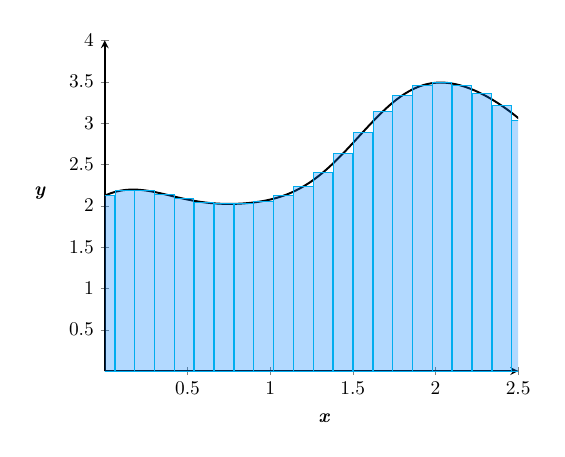
\begin{tikzpicture}[scale=0.7,
    declare function={
    % f(\x)=(\x^2)+9*\x+7;
        f(\x)=2+cos(deg(\x-2))+cos(deg(3*\x))/2+sin(cos(5*\x))/8 + cos(deg(7*\x))/28;
    }
]
\begin{axis}[
    axis lines = middle,
    xtick ={0.5, 1.0, 1.5, 2.0, 2.5, 3.0, 3.5},
    ytick ={0, 0.5, 1, 1.5, 2.0, 2.5, 3, 3.5, 4, 4.5, 5, 5.5},
    % xticklabels = {$a=x_0$,$x_1$,$x_2$,$x_3$, $\ldots$, $x_{n-1}$,$x_n=b$},
    ymin = 0,
    ymax = 4,
    xmin = 0,
    xmax = 2.5,
    x=3cm,y=1.5cm,
    axis line style = thick,
    xlabel style={at={(.5,0)},above right,yshift=-30pt},
    ylabel style={at={(0,.5)},above right,xshift=-40pt},
    xlabel={$\emph{\textbf{x}}$},
    ylabel={$\emph{\textbf{y}}$},
    % extra x ticks={1.3,1.85,2.2,2.7,3.2,3.75}
]

\addplot [
    % domain=1:4,
    samples=300,
    % line width=1pt,
    % fill=red, draw=none,
    % fill opacity=0.1
] {f(x)} \closedcycle;

\addplot [
    domain=0:5,
    samples=300,
    line width = 1pt, black] {f(x)};

\addplot[ybar, bar width=10pt, domain=1:4,samples at={0, 0.12, 0.24, 0.36, 0.48, 0.60, 0.72, 0.84, 0.96, 1.08, 1.20, 1.32, 1.44, 1.56, 1.68, 1.80, 1.92, 2.04, 2.16, 2.28, 2.40, 2.52, 2.64, 2.76, 2.88, 3.00, 3.12, 3.24, 3.36, 3.48}, fill=blue!50!cyan,fill opacity=0.3, draw=cyan]
  {f(x)};
\end{axis}
\end{tikzpicture}
\end{center}
\caption{Midpoint-Riemann Approximation of a Function}
\label{fig:riemannf}
\end{figure}

Design the \ttt{double circleArea(double r, double delta)} method, which receives a radius $r$ and a delta $\Delta$. It computes (and returns) a left/right-Riemann approximation of the area of a circle. Hint: if you compute the left/right-Riemann approximation of one quadrant, you can very easily obtain an approximation of the total circle area. We illustrate this hint in Figure~\ref{fig:circlearea} where $\Delta=0.5$ and its radius $r=2$. Note that the approximated area will vary based on the chosen Riemann approximation.\footnote{A left-Riemann sum over-approximates the area, whereas a right-Riemann sum provides an under-approximation. A midpoint approximation uses the average between the left and right approximations.} Further note that no calculus knowledge is necessary to solve this exercise.\footnote{This exercise comes directly from~\Citep{pocs}. Thanks, past me! Further thanks to Chandana Ariyawansa for the problem.}

\begin{figure}[H]
\begin{center}
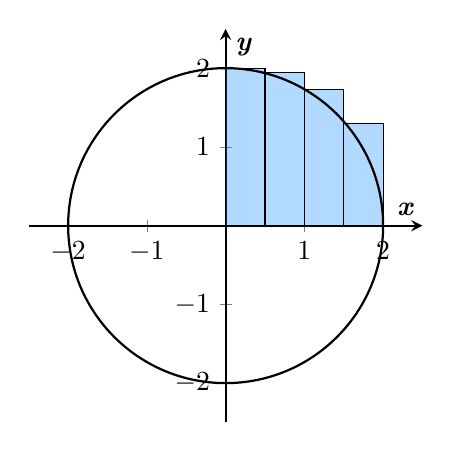
\begin{tikzpicture}
\begin{axis}[
    axis lines = middle,
    xtick ={-3,-2,-1,0,1,2,3},
    ytick ={-3,-2,-1,0,1,2,3},
    % xticklabels = {$a=x_0$,$x_1$,$x_2$,$x_3$, $\ldots$, $x_{n-1}$,$x_n=b$},
    ymin = -2.5,
    ymax = 2.5,
    xmin = -2.5,
    xmax = 2.5,
    x=1cm,y=1cm,
    axis line style = thick,
    xlabel={$\emph{\textbf{x}}$},
    ylabel={$\emph{\textbf{y}}$},
    % extra x ticks={1.3,1.85,2.2,2.7,3.2,3.75}
]
\end{axis}

  \draw[fill=blue!50!cyan,fill opacity=0.3] (2.5,2.5) rectangle (3,4.5);
  \draw[fill=blue!50!cyan,fill opacity=0.3] (3.0,2.5) rectangle (3.5,4.44);
  \draw[fill=blue!50!cyan,fill opacity=0.3] (3.5,2.5) rectangle (4.0,4.23);
  \draw[fill=blue!50!cyan,fill opacity=0.3] (4,2.5) rectangle (4.5,3.80);
\draw[thick] (2.5,2.5) circle (2);
\end{tikzpicture}

\end{center}
\caption{Left-Riemann Approximation of a Function}
\label{fig:circlearea}
\end{figure}

\newpage %ugh
\myexercise{2}{chapter-crl}{In 1964,~\Citet{willans} derived the following formula for computing the $n^\text{th}$ prime number:}

\[
p_n = 1 + \sum_{i=1}^{2^n}\left\lfloor\left(\frac{n}{\sum_{j=1}^{i}{\left\lfloor{\left({\cos{\frac{(j-1)! + 1}{j}\pi}}\right)^2}\right\rfloor}}\right)^{1/n}\right\rfloor
\]

While this looks frightening, it is actually straightforward and requires no conditionals. We know that `$n!$' is the factorial of some integer~$n$. The summation, $\sum_{j=1}^{n}{f(i)}$ is, effectively, a loop from $j=1$ to $n$, inclusive, which sums the value returned from~$f(i)$. Finally, $\left\lfloor{n}\right\rfloor$ computes the floor of a number~$n$, which is the next-closest integer to~$n$. E.g., the floor of $3.7$ is $3$. Use this formula to design the \ttt{int nthPrime(int n)} method, which returns the $n^\text{th}$ prime number. You \emph{must} use this formula exactly as specified.

\myexercise{3}{chapter-crl}{Speech-to-text software plays a significant role in accessibility for those who may not be able to type quickly or at all. Design the \ttt{String speechToText(String s)} method that, when given a ``speech string'', returns the corresponding text. A speech string, in this context, is a string spoken, in English, by a person, which may or may not contain punctuation. If a speech string contains a word that represents punctuation, e.g., \ttt{"period"}, \ttt{"question mark"}, encode this punctuation in the returned text. For example, \ttt{speechToText("hello period how are you question mark")} returns the string \ttt{"Hello. How are you?"}. You should also account for quotations, e.g., \ttt{speechToText\-("hello quote how are you question mark unquote")} returns the string \ttt{Hello. "how are you?"}.}